% Compile with:
% latexmk -pdf -pvc -interaction=nonstopmode
%\documentclass[aspectratio=169,draft]{beamer}
\documentclass[aspectratio=169,draft]{beamer}
\usetheme{UniBern}

\title{How to study the internals of +100 human teeth with X-ray microtomography}
\author{David Haberthür}
\date{November 12, 2020 | Internal seminar at the Institute of Anatomy}

%\includeonlyframes{current}
%then....
%\begin{frame}[label=current]
%\end{frame}

\usepackage[detect-all=true,
	range-phrase=--,
	range-units=single,
	binary-units=true,
	per-mode=symbol,
	per-symbol=/]{siunitx}
\usepackage{xspace}
\usepackage[missing=main]{gitinfo2} % GitHub Actions don't pull in the commit hash, so we just show the main branch as placeholder
\usepackage[backend=biber,
	style=numeric,
	url=false,
	maxnames=1,
	sorting=none
	]{biblatex}
%\addbibresource{~/P/Documents/library.bib}
\addbibresource{~/Documents/library.bib}
\usepackage{ccicons}
\usepackage{animate}
\usepackage{standalone} % for CT animations
\usepackage{tikz}
	\usetikzlibrary{spy}
	\tikzset{shadowed/.style={preaction={transform canvas={shift={(1pt,-1pt)}},draw=ubRed}}}
\usepackage{shadowtext}  % for the shadowed scalebar
	\shadowoffset{1pt}
	\shadowcolor{ubRed}
\usepackage[absolute,overlay]{textpos} %for the \source* command	
\usepackage{fontawesome5}
\usepackage{standalone}
\usepackage[version=4]{mhchem}
\usepackage{listings}
	\lstset{frame=single,
	basicstyle=\tiny\ttfamily
	}
\usepackage{microtype}

% Some often used abbreviations/commands
\newcommand{\everyframe}{111} % use only every nth frame for the animations
\newcommand{\imwidth}{\linewidth}% set global image width
\newcommand{\imheight}{0.618\paperheight}% set global image height
\newlength\imagewidth% needed for scalebars
\newlength\imagescale% needed for scalebars
\newcommand{\uct}{\si{\micro}CT\xspace}% make our life easier
\newcommand{\eg}{e.\,g.\xspace}%
\newcommand{\ie}{i.\,e.\xspace}%

% Define complementary colors to ubRed
\definecolor{ubRedComplementary1}{HTML}{00a1e6}
\definecolor{ubRedComplementary2}{HTML}{00e645}

% Acknowledge images just below them
% Based on https://tex.stackexchange.com/a/282637/828
\newcommand{\source}[2]{%
	% Print out (short) link under image, with small text
	\raisebox{-1.618ex}{%
		\makebox[0pt][r]{%
			\scriptsize\href{http://#1}{#1} #2%
			}%
		}%
	}%
\newcommand{\sourcecite}[2]{%
	% Cite (an image from) a reference
	\raisebox{-1.618ex}{%
		\makebox[0pt][r]{%
			\scriptsize From \cite{#1}, #2%
			}%
		}%
	}%
\newcommand{\sourcelink}[3]{%
	% Make the source command an \href{link}{text}
	\raisebox{-1.618ex}{%
		\makebox[0pt][r]{%
			\scriptsize\href{http://#1}{#2}, #3%
			}%
		}%
	}%

% Define us a custom footer *with* progress bar, based on https://tex.stackexchange.com/a/59749/828
\makeatletter
\def\progressbar@progressbar{} % the progress bar
\newcount\progressbar@tmpcounta% auxiliary counter
\newcount\progressbar@tmpcountb% auxiliary counter
\newdimen\progressbar@pbht %progressbar height
\newdimen\progressbar@pbwd %progressbar width
\newdimen\progressbar@rcircle % radius for the circle
\newdimen\progressbar@tmpdim % auxiliary dimension
\progressbar@pbwd=\linewidth
\progressbar@rcircle=1.5pt
\def\progressbar@progressbar{%
	\progressbar@tmpcounta=\insertframenumber
	\progressbar@tmpcountb=\inserttotalframenumber
	\progressbar@tmpdim=\progressbar@pbwd
	\multiply\progressbar@tmpdim by \progressbar@tmpcounta
	\divide\progressbar@tmpdim by \progressbar@tmpcountb
	\par%
	\begin{tikzpicture}%
		\draw[ubGrey] (0,0) -- ++ (\progressbar@pbwd,0);
		\filldraw[ubGrey] (\the\dimexpr\progressbar@tmpdim-\progressbar@rcircle\relax,.5\progressbar@pbht) circle (\progressbar@rcircle);
	\end{tikzpicture}%
	v. \href{https://github.com/habi/20201112_Anatomie_Seminar/commit/\gitHash}{\gitAbbrevHash}\xspace|\xspace%
	p.\xspace\insertframenumber/\inserttotalframenumber%
%	\hspace*{4ex}%
	\vspace{0.7ex}
	\par%
}
\addtobeamertemplate{footline}{}
{%
	\begin{beamercolorbox}[wd=\paperwidth,center]{white}%
		\progressbar@progressbar%
	\end{beamercolorbox}%
}
\makeatother

% Format bibliography for beamer
% http://tex.stackexchange.com/a/10686/828
\renewbibmacro{in:}{}
% http://tex.stackexchange.com/a/13076/828
\AtEveryBibitem{%
	\clearfield{journaltitle}
	\clearfield{pages}
	\clearfield{volume}
	\clearfield{number}
	\clearname{editor}
	\clearfield{issn}
	\clearfield{year}
}
% No parentheses around the (now empty) year: https://tex.stackexchange.com/a/147537/828
\renewcommand{\bibopenparen}{\addcomma\addspace}
\renewcommand{\bibcloseparen}{\addcomma\addspace}

% open in fullscreen
\hypersetup{pdfpagemode=FullScreen}

% Move the text down a bit
% THIS IS A BIG HACK, IT SHOULD BE FIXED IN THE TEMPLATE
\addtobeamertemplate{frametitle}{}{\vspace*{0.75em}}

% Small citations as footnotes
\setbeamerfont{footnote}{size=\tiny}

\begin{document}
% No footline on the title page
% http://tex.stackexchange.com/a/18829/828 helps us to achieve that
{%
	\setbeamertemplate{footline}{}%
	\begin{frame}%
		\maketitle
	\end{frame}%
}

\begin{frame}
	\frametitle{Grüessech!}
	\begin{itemize}
		\item David
		\begin{itemize}
			\item Physicist by trade
			\item \href{https://boris.unibe.ch/2619/}{PhD in high resolution imaging of the lung}
			\item Post-Doc I: \href{https://www.psi.ch/sls/tomcat/}{TOMCAT}, \href{https://www.psi.ch/sls/}{Swiss Light Source}, \href{https://www.psi.ch/}{Paul Scherrer Institute}
			\item Post-Doc II: \uct-group, Topographic and clinical Anatomy with Ruslan Hlushchuk, Oleksiy-Zakhar Khoma and Tim Hoessly
		\end{itemize}
		\item Biomedical imaging and research
		\begin{itemize}
			\item microangioCT~\cite{Hlushchuk2018}: Tumor vasculature, angiogenesis in the heart, musculature and bones
			\item Physiology: Zebrafish musculature and gills~\cite{MesserliAaldijk2020}			
			\item Computer science: Automate \emph{all} the things~\cite{Haberthur2020}
			\item Lung tumor detection and classification
		\end{itemize}
	%\item<1-> SkyScan 1172 \& 1272 \uncover<2->{\& 2214}							
	\end{itemize}
\end{frame}

\begin{frame}
	\frametitle{Contents}
	\tableofcontents
\end{frame}

\section{Overview}
\begin{frame}
	\frametitle{Biomedical imaging}
	\begin{columns}
		\begin{column}{0.4\linewidth}
			\begin{itemize}
				\item<1->Medical research
				\item<1->Non-destructive insights into the samples
				\item<2->(Small) Biological samples
			\end{itemize}
		\end{column}
		\begin{column}{0.6\linewidth}
			\centering
			\only<1-2>{%
				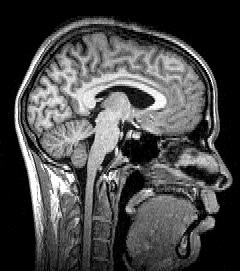
\includegraphics[height=\imheight]{./images/Sagittal_brain_MRI}
				\source{w.wiki/7g4}{\ccbysa}
			}
			\only<3>{%
				\begin{tikzpicture}[remember picture,overlay]%
					\node at (current page.center){%
						\animategraphics[loop,autoplay,width=\paperwidth,every=\everyframe]{24}{./movies/mouse_skull/mouse_skull}{000}{236}%
					};%
				\end{tikzpicture}%
			}
		\end{column}
	\end{columns}
\end{frame}
	
\section{(micro)Tomography}
\begin{frame}
	\frametitle{Scale}
	\centering
	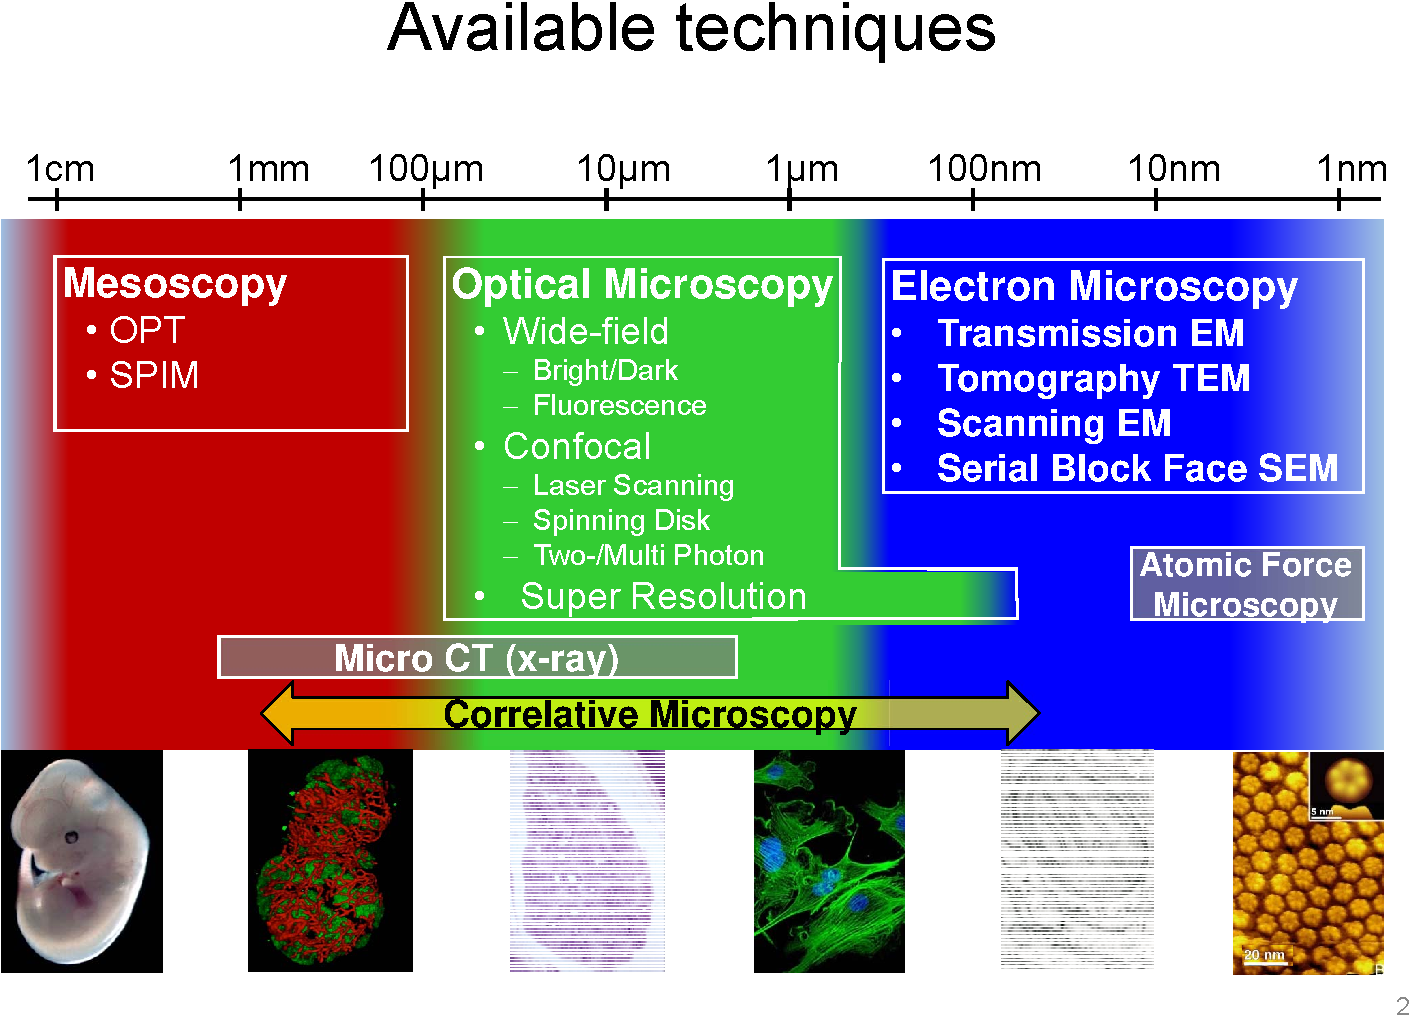
\includegraphics[height=\imheight]{./images/AnatomySeminarYuryBelyaev-cropped}%
	\sourcelink{www.mic.unibe.ch/organisation.php}{Yury Belyaev, MIC}{slide from internal seminar presentation}
\end{frame}

\begin{frame}
	\frametitle{CT-Scanner}
	\centering
	\animategraphics[loop,autoplay,height=\imheight,every=\everyframe]{24}{./movies/ct-scanner/ct-scanner0}{001}{480}%
	\source{youtu.be/2CWpZKuy-NE}{}%
	\note{From \href{https://www.bruker.com/products/microtomography/micro-ct-for-sample-scanning/x-ray-micro-ct-microtomography.html}:
		Micro computed tomography or micro-CT is x-ray imaging in 3D, by the same method used in hospital CT (or CAT) scans, but on a small scale with massively increased resolution.
		It really represents 3D microscopy, where very fine scale internal structure of objects is imaged non-destructively.
		No sample preparation, no staining, no thin slicing - a single scan will image your sample's complete internal 3D structure at high resolution, plus you get your intact sample back at the end!}
\end{frame}

\section{Why \uct?}
\renewcommand{\imwidth}{\columnwidth}
\begin{frame}
	\frametitle{Why \uct?}
	\begin{columns}
		\begin{column}{0.49\linewidth}
			% https://www.cancerimagingarchive.net/nbia-search/?saved-cart=nbia-76761575299081509
			\only<1-4>{%
				\pgfmathsetlength{\imagewidth}{\imwidth}%
				\pgfmathsetlength{\imagescale}{\imagewidth/512}%
				\def\x{316}% scalebar-x starting at golden ratio of image width of 512px = 316
				\def\y{361}% scalebar-y at 90% of image height of 401px = 361
				\begin{tikzpicture}[x=\imagescale,y=-\imagescale]
					\node[anchor=north west, inner sep=0pt, outer sep=0pt] at (0,0) {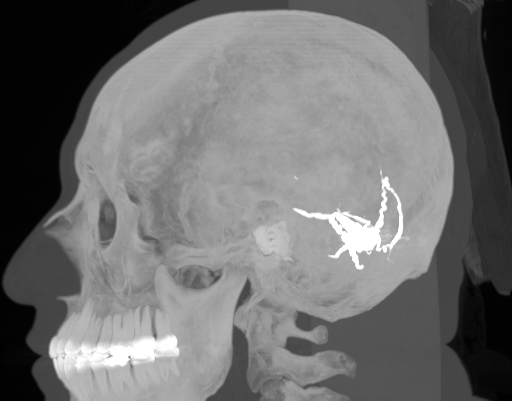
\includegraphics[width=\imagewidth]{./images/comparison/MAX_human}};
					% 512.000px = 250.0096mm -> 100px = 48830.000um -> 1.024px = 500um, 0.205px = 100um
					%\draw[|-|,blue,thick] (0,200) -- (512,200) node [sloped,midway,above,fill=white,semitransparent,text opacity=1] {\SI{250.0096}{\milli\meter} (512px) TEMPORARY!};
					\draw[|-|,white,shadowed] (\x,\y) -- (\x+102.4,\y) node [midway,above] {\shadowtext{\SI{5}{\centi\meter}}};
				\end{tikzpicture}%
			}%
			\only<5>{%
				\pgfmathsetlength{\imagewidth}{\imwidth}%
				\pgfmathsetlength{\imagescale}{\imagewidth/512}%
				\def\x{316}% scalebar-x starting at golden ratio of image width of 512px = 316
				\def\y{361}% scalebar-y at 90% of image height of 401px = 361
				\def\mag{5}% magnification of inset
				\def\size{100}% size of inset
				\begin{tikzpicture}[x=\imagescale,y=-\imagescale,spy using outlines={rectangle,magnification=\mag,size=\size,connect spies}]
					\node[anchor=north west, inner sep=0pt, outer sep=0pt] at (0,0) {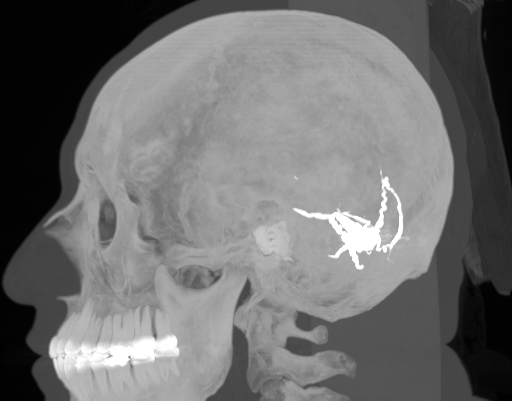
\includegraphics[width=\imagewidth]{./images/comparison/MAX_human}};
					\spy [red] on (102,342) in node at (256,201) [anchor=center];
					% 512.000px = 250.0096mm -> 100px = 48830.000um -> 1.024px = 500um, 0.205px = 100um
					\draw[|-|,white,shadowed] (\x,\y) -- (\x+102.4,\y) node [midway,above] {\shadowtext{\SI{5}{\centi\meter}}};
				\end{tikzpicture}%
			}%
			\renewcommand{\imwidth}{0.1554\columnwidth}%			
			\only<6>{%
				\centering
				\pgfmathsetlength{\imagewidth}{\imwidth}%
				\pgfmathsetlength{\imagescale}{\imagewidth/512}%
				\def\x{316}% scalebar-x starting at golden ratio of image width of 512px = 316
				\def\y{361}% scalebar-y at 90% of image height of 401px = 361
				\begin{tikzpicture}[x=\imagescale,y=-\imagescale]
					\node[anchor=north west, inner sep=0pt, outer sep=0pt] at (0,0) {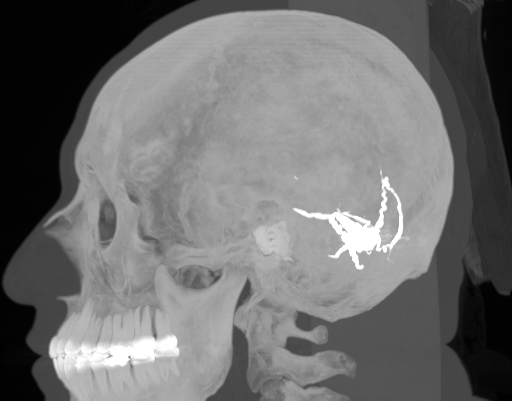
\includegraphics[width=\imagewidth]{./images/comparison/MAX_human}};
					% 512.000px = 250.0096mm -> 100px = 48830.000um -> 1.024px = 500um, 0.205px = 100um
					\draw[|-|,white,shadowed] (\x,\y) -- (\x+102.4,\y) node [midway,above] {\shadowtext{\SI{5}{\centi\meter}}};
				\end{tikzpicture}%
			}%			
			\sourcecite{Clark2013}{Subject \emph{C3L-02465}}
		\end{column}%
		\begin{column}{0.49\linewidth}
			\only<1>{%
				\pgfmathsetlength{\imagewidth}{\imwidth}%
				\pgfmathsetlength{\imagescale}{\imagewidth/3295}%
				\def\x{2036}% scalebar-x starting at golden ratio of image width of 3295px = 2036
				\def\y{1343}% scalebar-y at 90% of image height of 1492px = 1343
				\begin{tikzpicture}[x=\imagescale,y=-\imagescale]
					\node[anchor=north west, inner sep=0pt, outer sep=0pt] at (0,0) {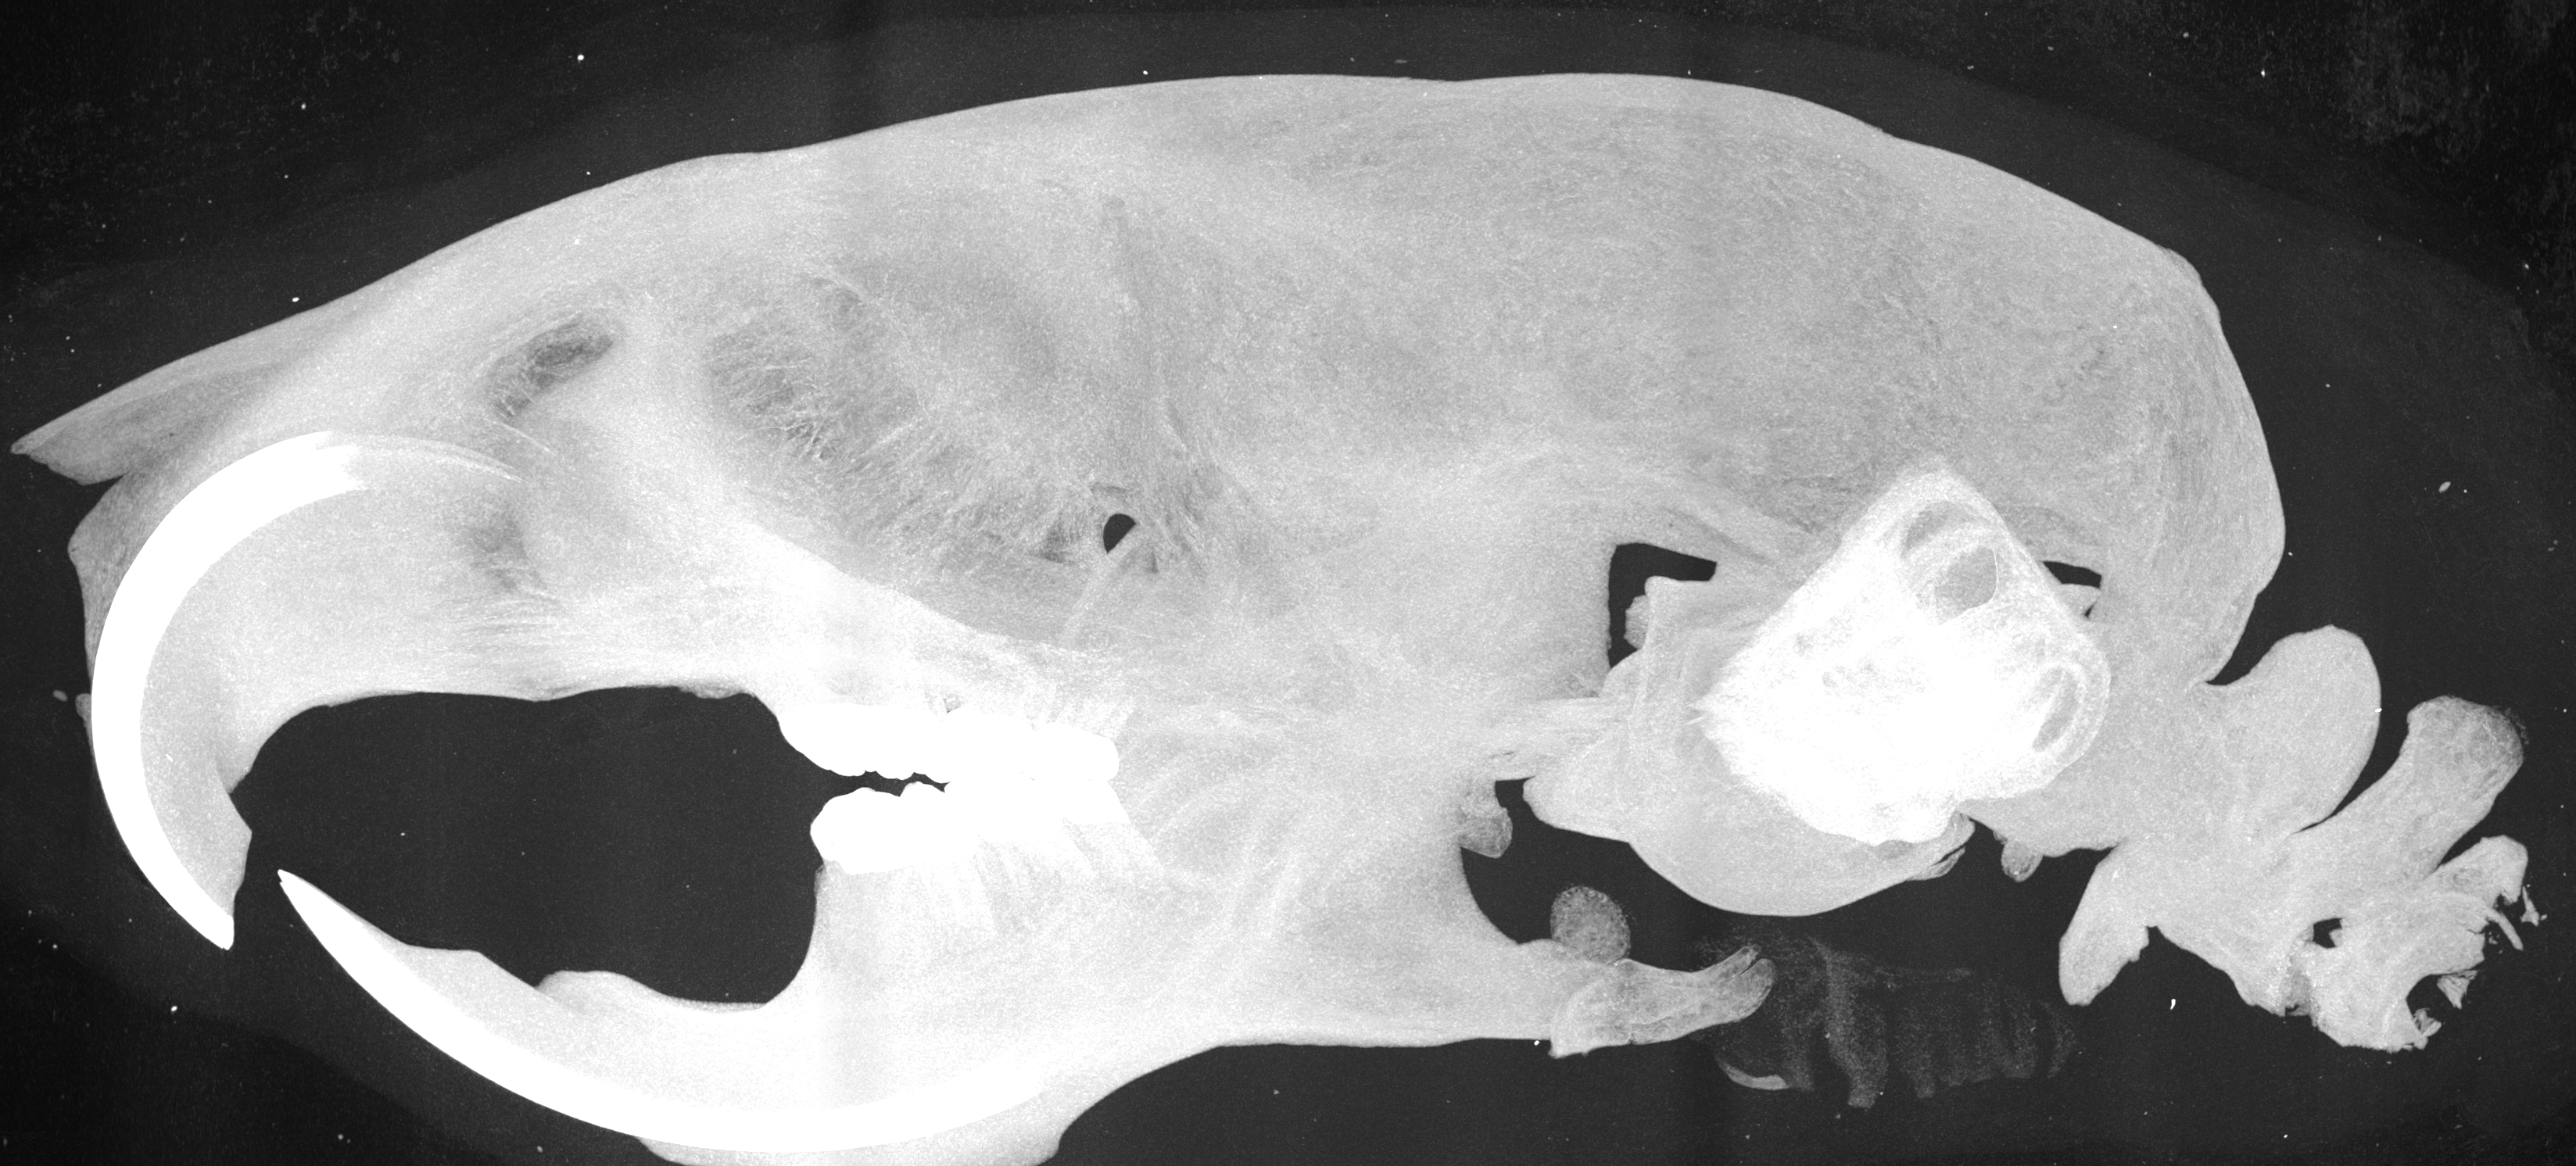
\includegraphics[width=\imagewidth]{./images/comparison/MAX_mouse}};
					% 3295.000px = 26.2282mm -> 100px = 796.000um -> 62.814px = 500um, 12.563px = 100um
					%\draw[|-|,blue,thick] (0,746) -- (3295,746) node [sloped,midway,above,fill=white,semitransparent,text opacity=1] {\SI{26.2282}{\milli\meter} (3295px) TEMPORARY!};
					\draw[|-|,white,shadowed] (\x,\y) -- (\x+628.14,\y) node [midway,above] {\shadowtext{\SI{5}{\milli\meter}}};
				\end{tikzpicture}%
			}%
			\renewcommand{\imwidth}{0.1\columnwidth}%
			\only<2>{%
				\centering
				\pgfmathsetlength{\imagewidth}{\imwidth}%
				\pgfmathsetlength{\imagescale}{\imagewidth/54}%
				\def\x{33}% scalebar-x starting at golden ratio of image width of 54px = 33
				\def\y{22}% scalebar-y at 90% of image height of 24px = 22
				\begin{tikzpicture}[x=\imagescale,y=-\imagescale]
					\node[anchor=north west, inner sep=0pt, outer sep=0pt] at (0,0) {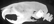
\includegraphics[width=\imagewidth]{./images/comparison/MAX_mouse_488umppx}};
					% 54.000px = 26.3682mm -> 100px = 48830.000um -> 1.024px = 500um, 0.205px = 100um
					%\draw[|-|,blue,thick] (0,12) -- (54,12) node [sloped,midway,above,fill=white,semitransparent,text opacity=1] {\SI{26.3682}{\milli\meter} (54px) TEMPORARY!};
					\draw[|-|,white,shadowed] (\x,\y) -- (\x+102.4,\y) node [midway,above] {\shadowtext{\SI{5}{\centi\meter}}};
					%\draw[color=red, anchor=south west] (0,24) node [fill=white, semitransparent] {Legend} node {Legend};
				\end{tikzpicture}%
			}%
			\renewcommand{\imwidth}{\columnwidth}
			\only<3>{%
				\centering
				\pgfmathsetlength{\imagewidth}{\imwidth}%
				\pgfmathsetlength{\imagescale}{\imagewidth/54}%
				\def\x{33}% scalebar-x starting at golden ratio of image width of 54px = 33
				\def\y{22}% scalebar-y at 90% of image height of 24px = 22
				\begin{tikzpicture}[x=\imagescale,y=-\imagescale]
					\node[anchor=north west, inner sep=0pt, outer sep=0pt] at (0,0) {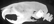
\includegraphics[width=\imagewidth]{./images/comparison/MAX_mouse_488umppx}};
					% 54.000px = 26.3682mm -> 100px = 48830.000um -> 1.024px = 500um, 0.205px = 100um
					%\draw[|-|,blue,thick] (0,12) -- (54,12) node [sloped,midway,above,fill=white,semitransparent,text opacity=1] {\SI{26.3682}{\milli\meter} (54px) TEMPORARY!};
					\draw[|-|,white,shadowed] (\x,\y) -- (\x+10.24,\y) node [midway,above] {\shadowtext{\SI{5}{\milli\meter}}};
					%\draw[color=red, anchor=south west] (0,24) node [fill=white, semitransparent] {Legend} node {Legend};
				\end{tikzpicture}%
			}%
			\only<4>{%
				\pgfmathsetlength{\imagewidth}{\imwidth}%
				\pgfmathsetlength{\imagescale}{\imagewidth/3295}%
				\def\x{2036}% scalebar-x starting at golden ratio of image width of 3295px = 2036
				\def\y{1343}% scalebar-y at 90% of image height of 1492px = 1343
				\begin{tikzpicture}[x=\imagescale,y=-\imagescale]
					\node[anchor=north west, inner sep=0pt, outer sep=0pt] at (0,0) {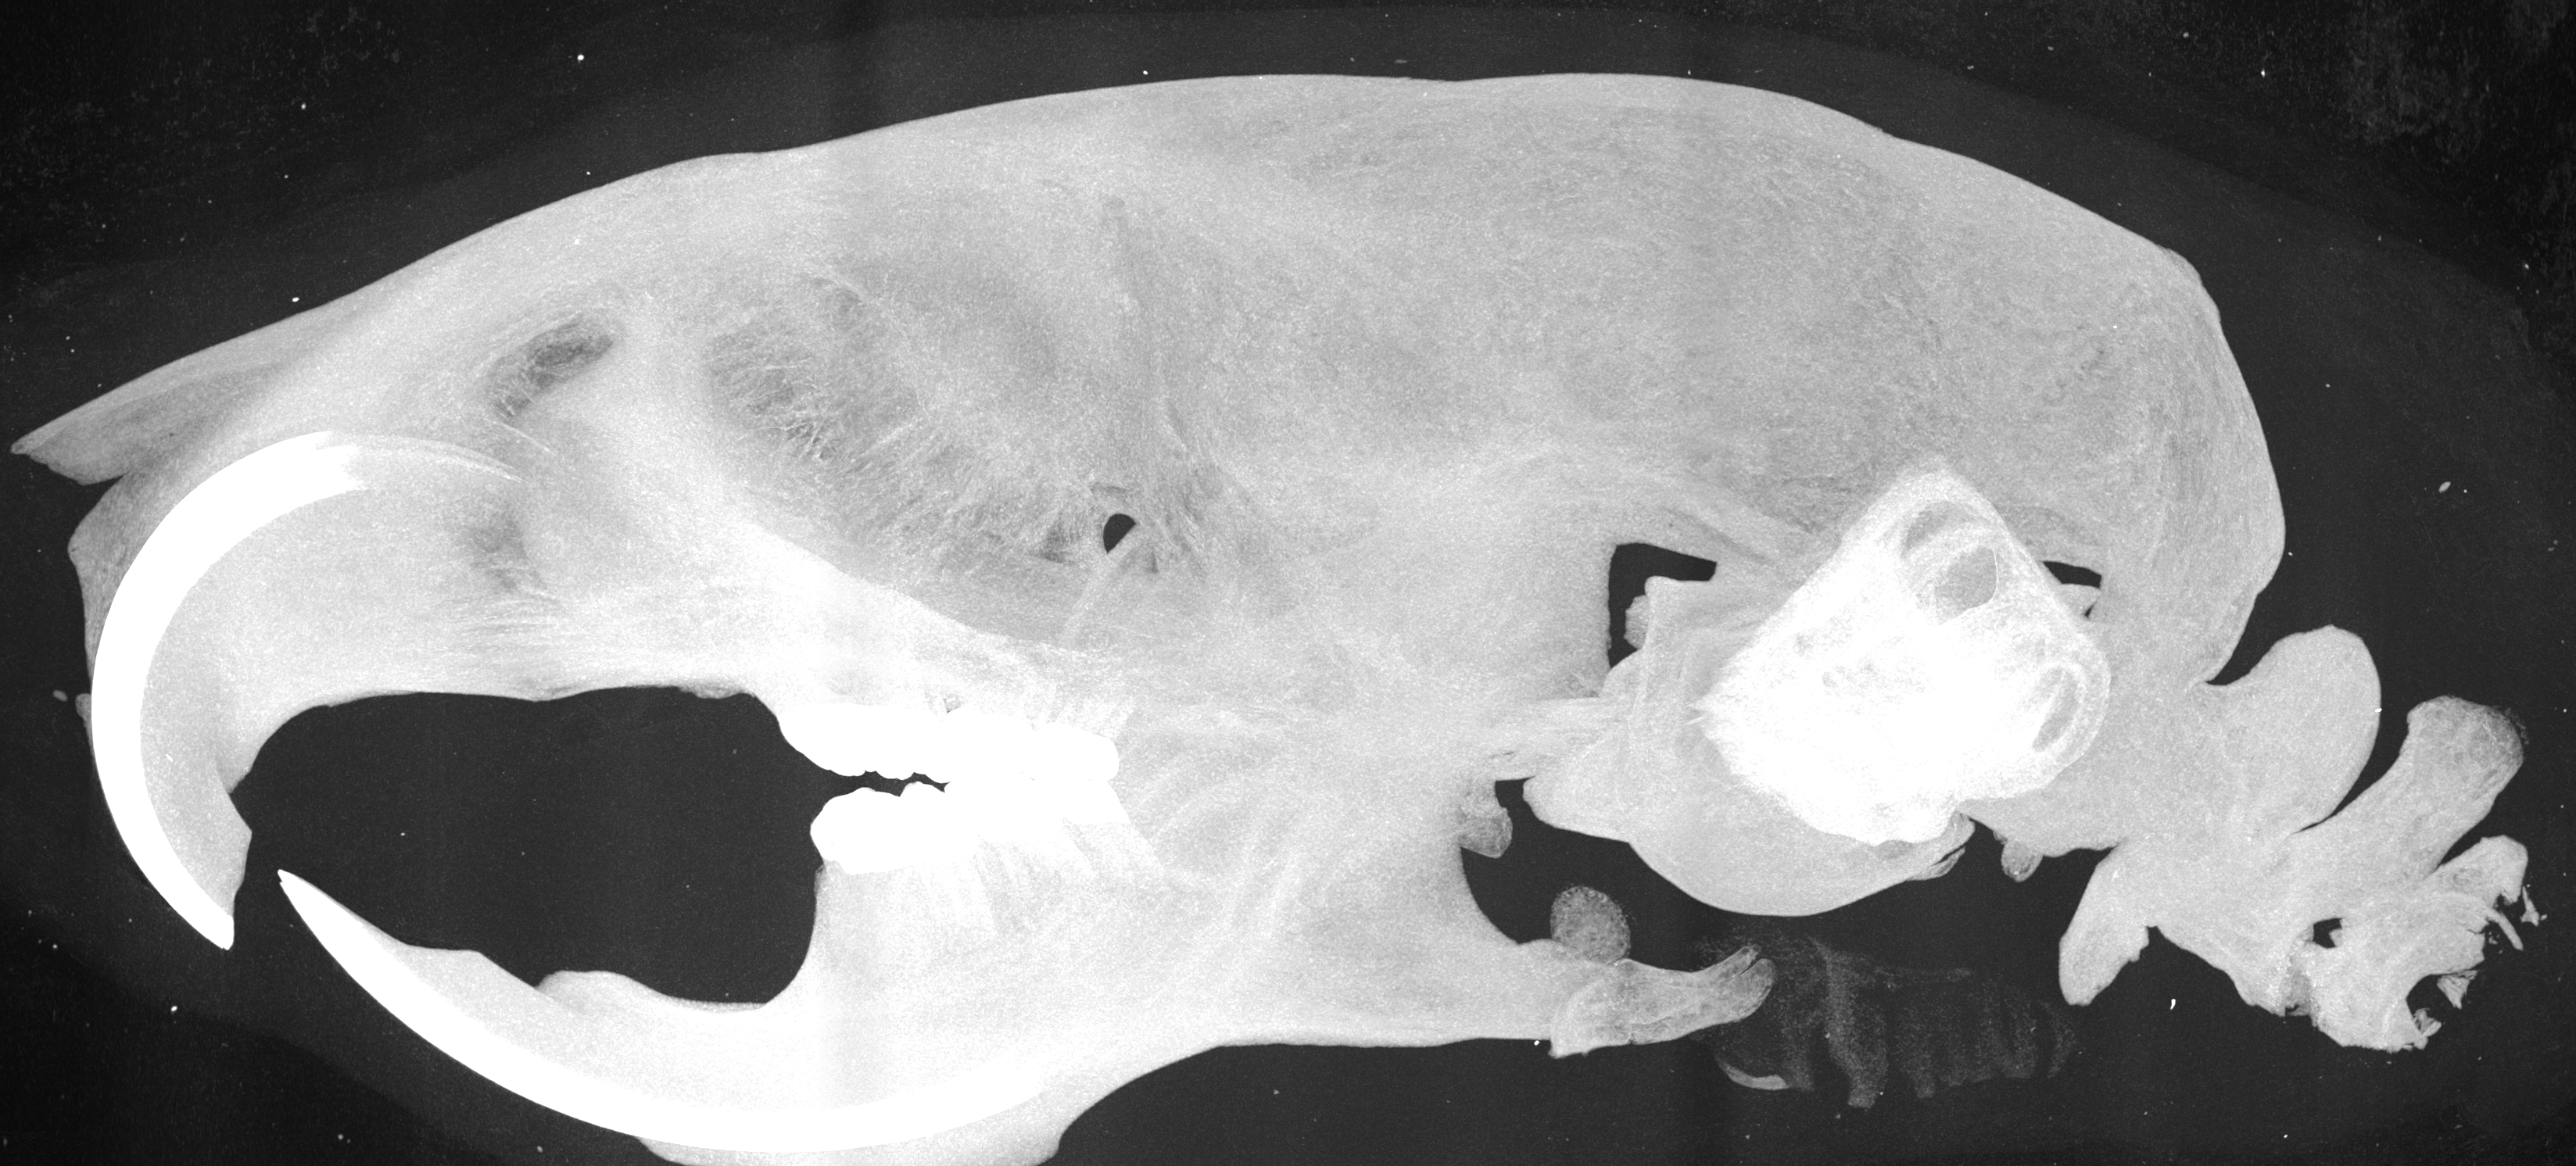
\includegraphics[width=\imagewidth]{./images/comparison/MAX_mouse}};
					% 3295.000px = 26.2282mm -> 100px = 796.000um -> 62.814px = 500um, 12.563px = 100um
					\draw[|-|,white,shadowed] (\x,\y) -- (\x+628.14,\y) node [midway,above] {\shadowtext{\SI{5}{\milli\meter}}};
				\end{tikzpicture}%
			}%
			\only<5>{%
				\pgfmathsetlength{\imagewidth}{\imwidth}%
				\pgfmathsetlength{\imagescale}{\imagewidth/3295}%
				\def\x{2036}% scalebar-x starting at golden ratio of image width of 3295px = 2036
				\def\y{1343}% scalebar-y at 90% of image height of 1492px = 1343
				\def\mag{5}% magnification of inset
				\def\size{100}% size of inset
				\begin{tikzpicture}[x=\imagescale,y=-\imagescale,spy using outlines={rectangle,magnification=\mag,size=\size,connect spies}]
					\node[anchor=north west, inner sep=0pt, outer sep=0pt] at (0,0) {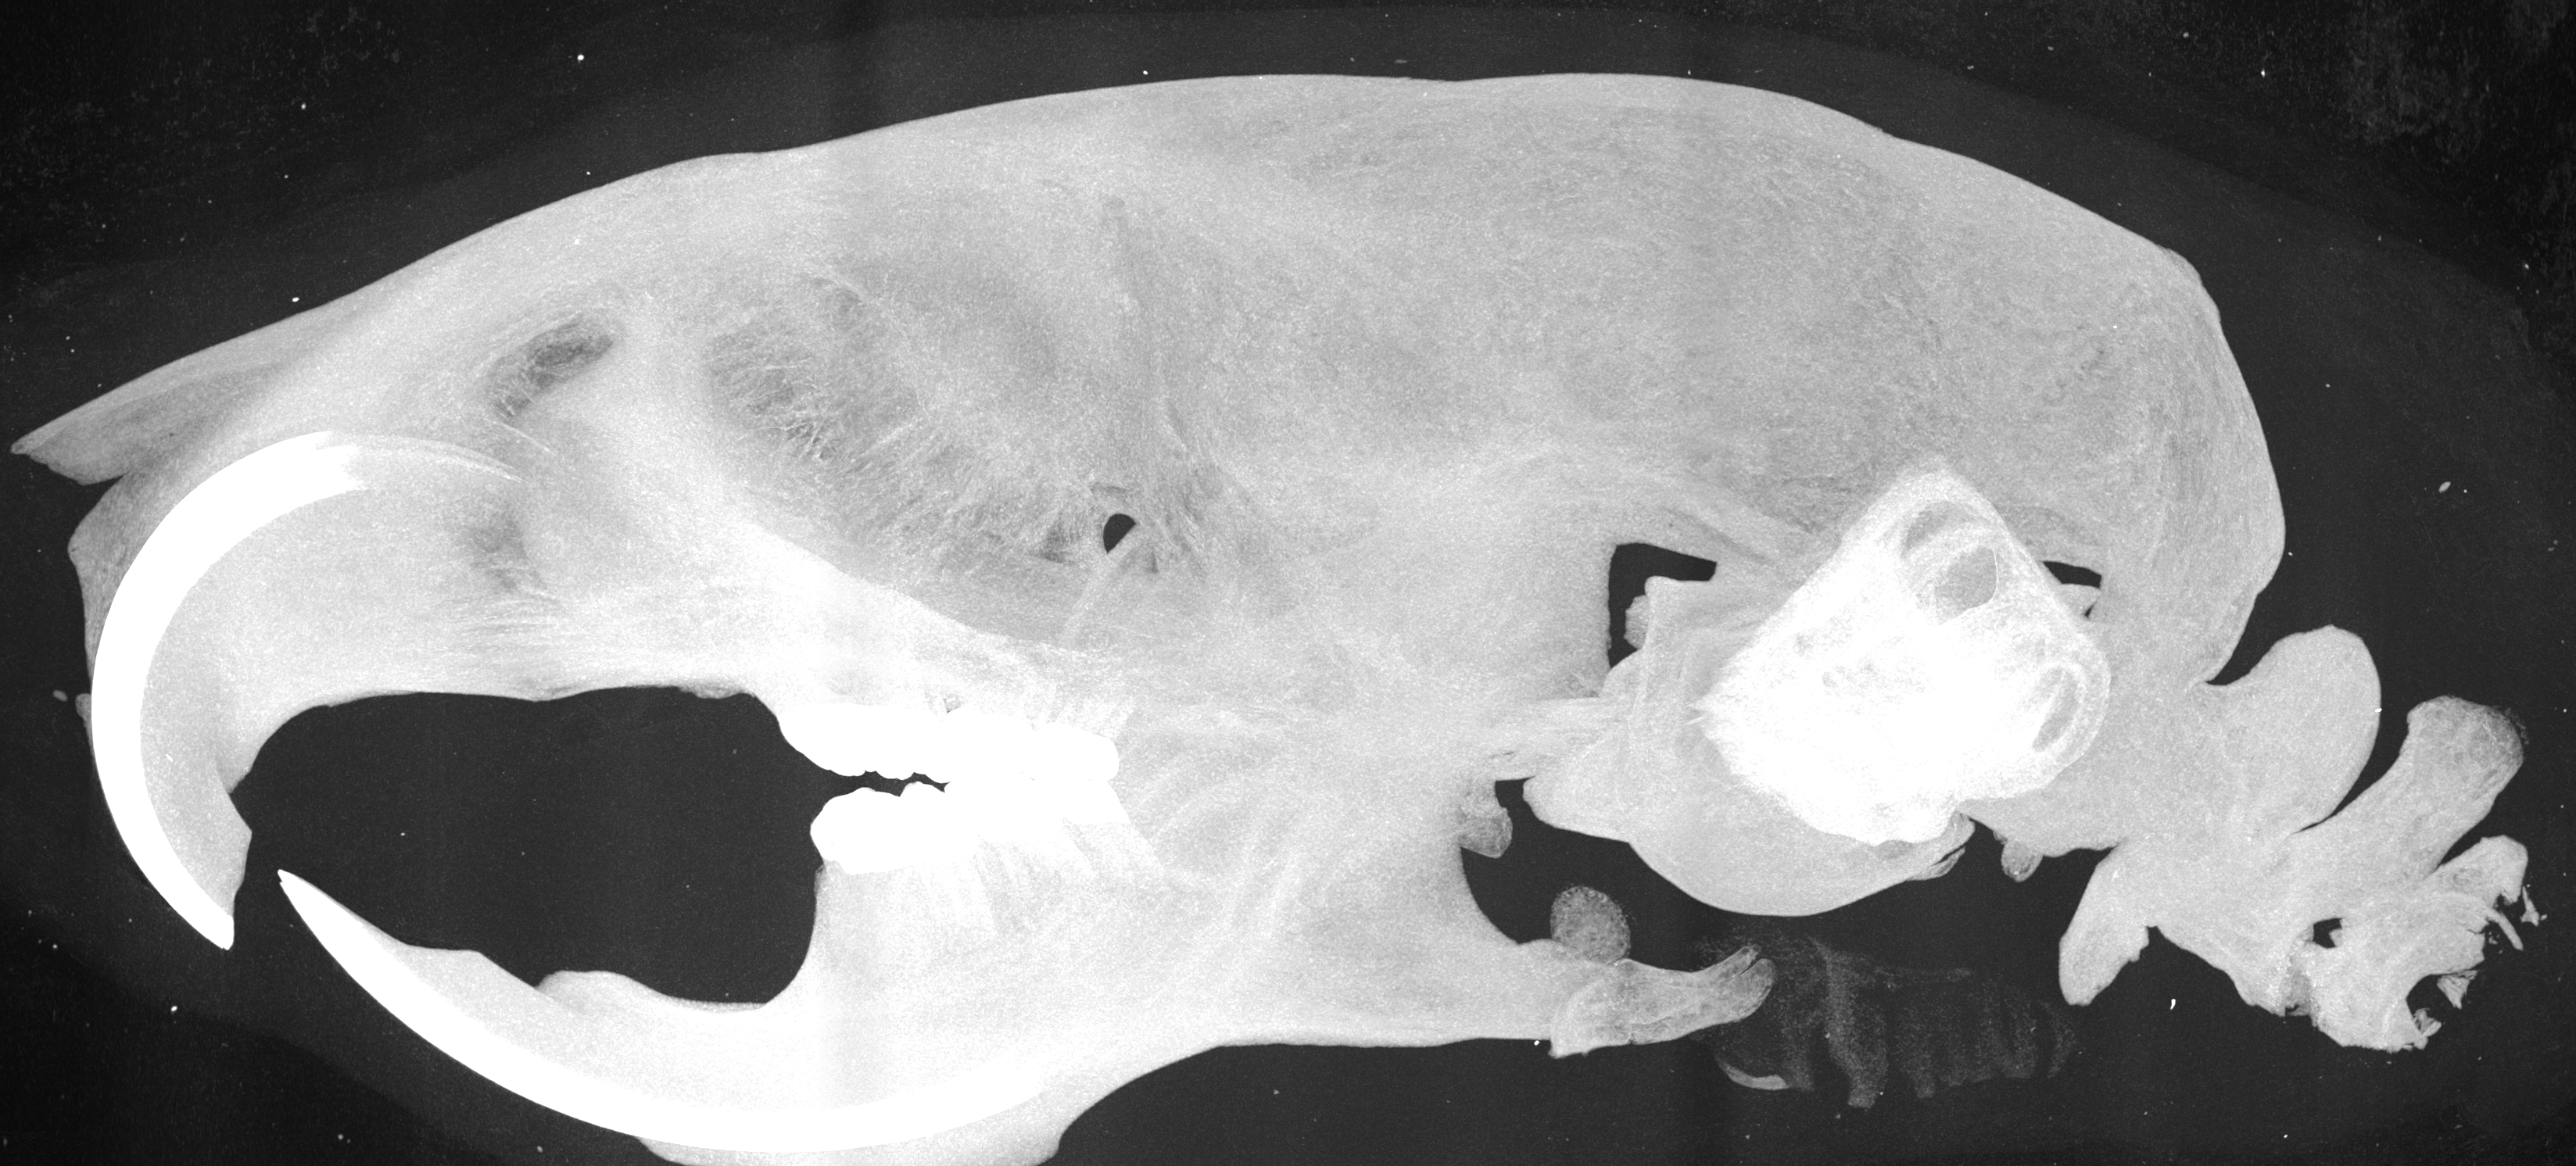
\includegraphics[width=\imagewidth]{./images/comparison/MAX_mouse}};
					\spy [red] on (352,1116) in node at (1648,746) [anchor=center];
					% 3295.000px = 26.2282mm -> 100px = 796.000um -> 62.814px = 500um, 12.563px = 100um
					\draw[|-|,white,shadowed] (\x,\y) -- (\x+628.14,\y) node [midway,above] {\shadowtext{\SI{5}{\milli\meter}}};
				\end{tikzpicture}%
			}%
			\only<6>{%
				\pgfmathsetlength{\imagewidth}{\imwidth}%
				\pgfmathsetlength{\imagescale}{\imagewidth/3295}%
				\def\x{2036}% scalebar-x starting at golden ratio of image width of 3295px = 2036
				\def\y{1343}% scalebar-y at 90% of image height of 1492px = 1343
				\begin{tikzpicture}[x=\imagescale,y=-\imagescale]
					\node[anchor=north west, inner sep=0pt, outer sep=0pt] at (0,0) {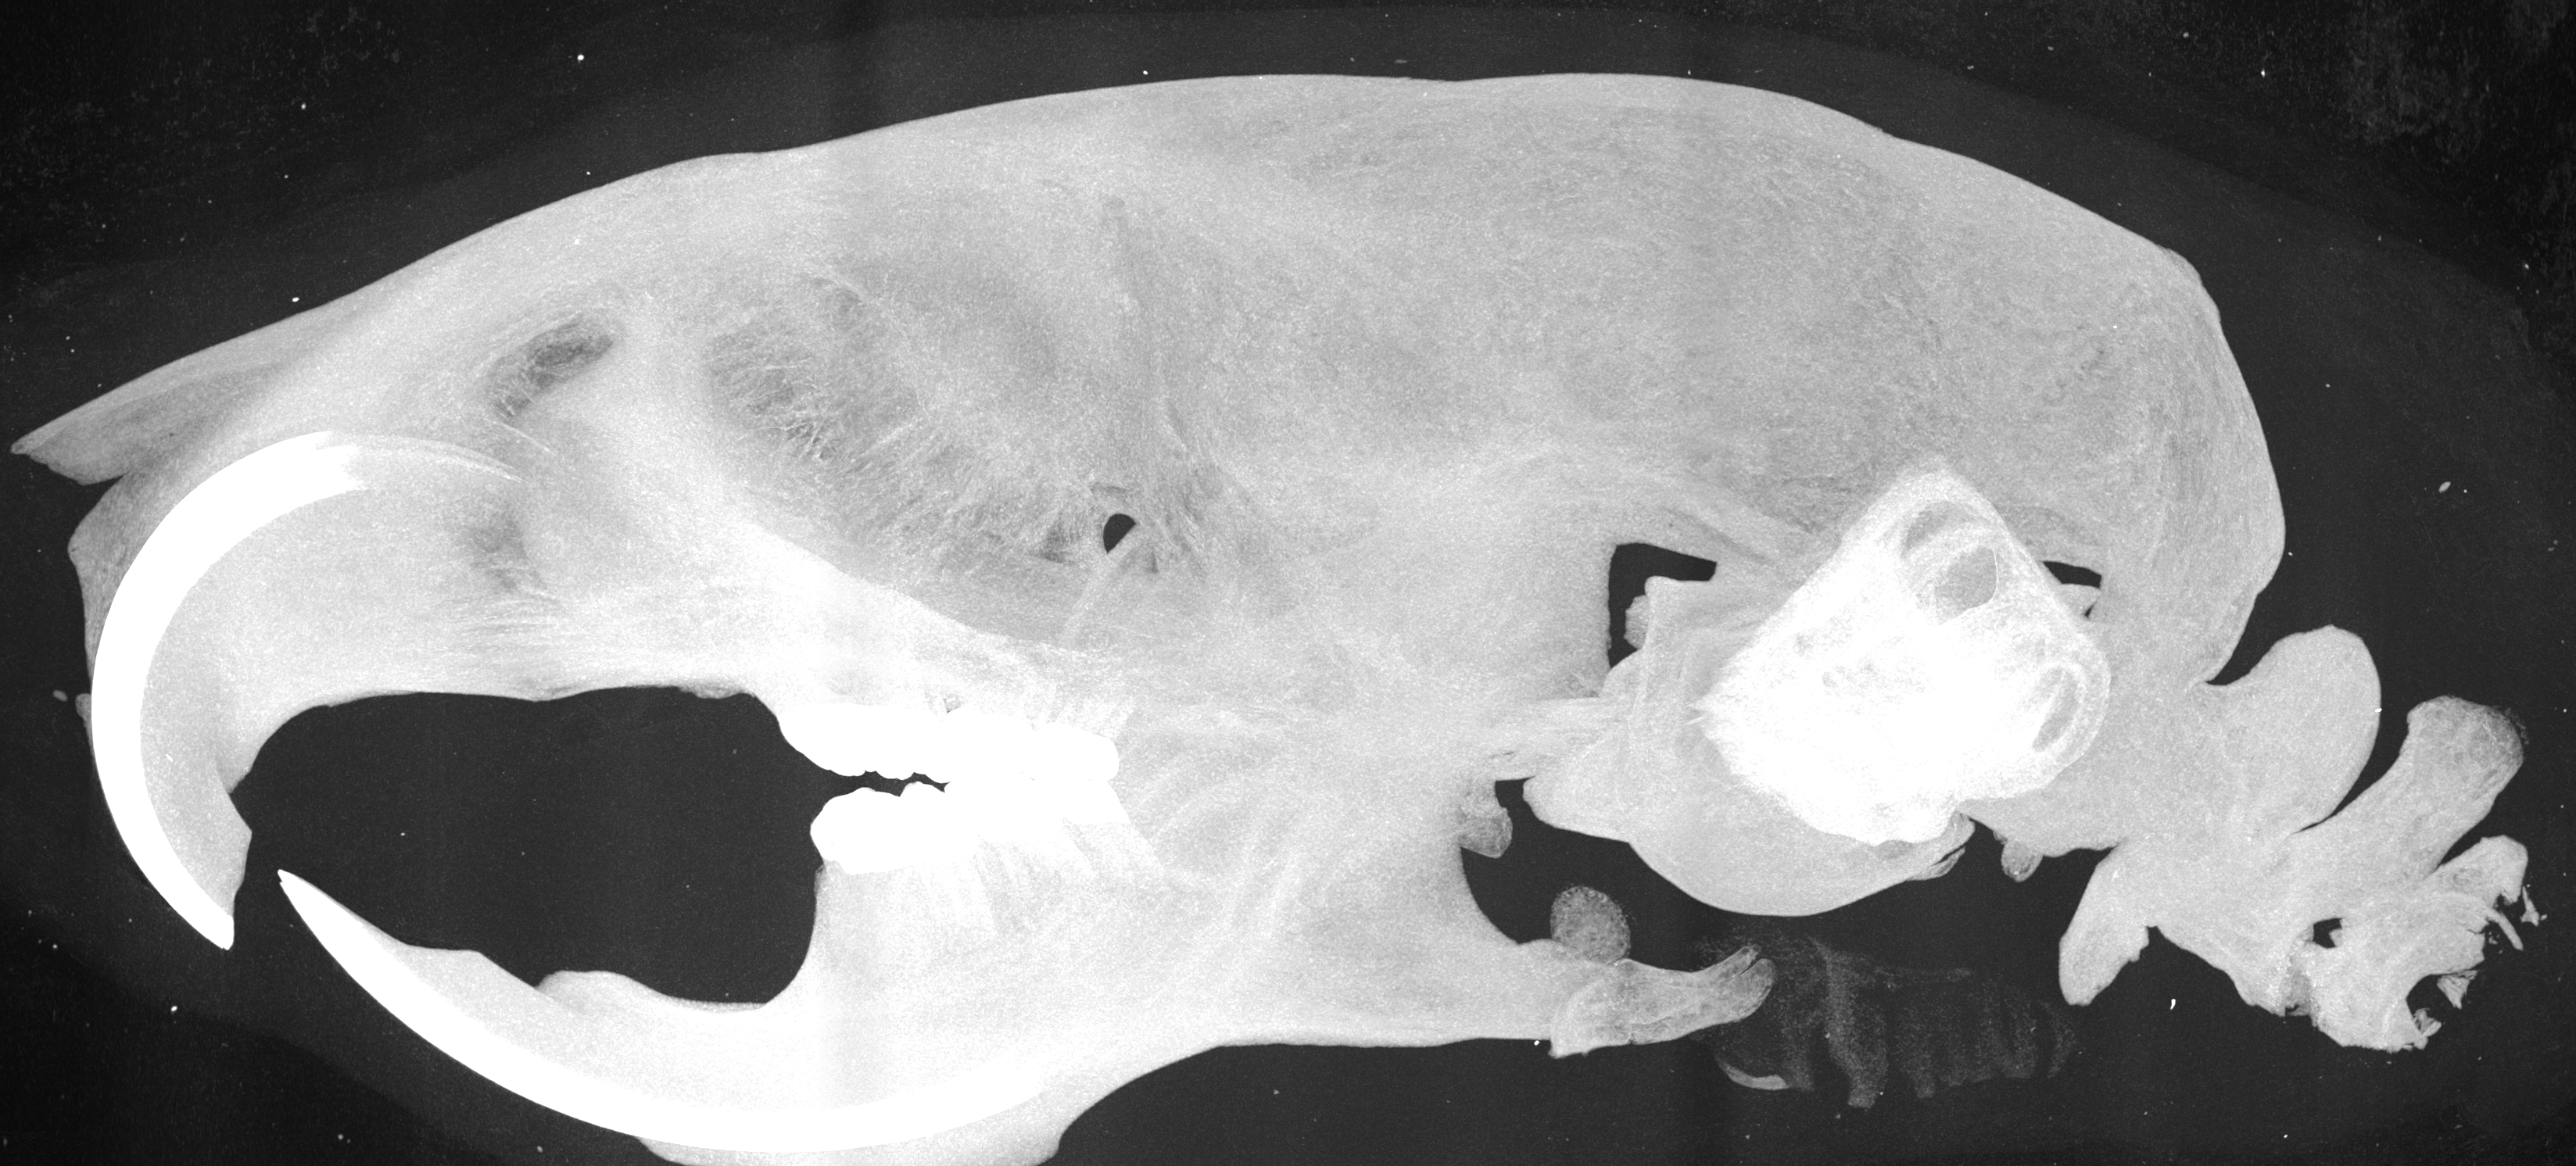
\includegraphics[width=\imagewidth]{./images/comparison/MAX_mouse}};
					% 3295.000px = 26.2282mm -> 100px = 796.000um -> 62.814px = 500um, 12.563px = 100um
					\draw[|-|,white,shadowed] (\x,\y) -- (\x+628.14,\y) node [midway,above] {\shadowtext{\SI{5}{\milli\meter}}};
				\end{tikzpicture}%
			}%
		\end{column}
	\end{columns}
\note{The human head scan was downloaded from the \href{https://www.cancerimagingarchive.net}{[Cancer Imaging Archive}{Cancer Imaging Archive}.
	We loaded the DICOM slices in Fiji, resliced it to show it from the side and then used to generate an MIP.
	According to the DICOM tags, the voxel size is \SI{0.4883x0.4883x0.625}{\milli\meter\cubed}, the image size is 512\(\times\)512 pixels.
	The mouse head is the same as shown in the early animation.
	The files from the early animation are resized 0.25 times, so we used the original dataset (Mouse1265\_Skull\_Gaby\_TKI\_7\_96um\_Al05\_2K) for a reslice and the generation of the MIP.
	The voxel size of the original data is 7.96 um, the image size is 3295\(\times\)1492 pixels, e.g. 26.32 mm.
	}
\end{frame}

\frametitle{Computed tomography}
\begin{frame}
	\frametitle{Machinery}
	\begin{columns}
		\begin{column}{0.39\linewidth}
			\begin{itemize}
				\item<1-> Hospital CT
				\begin{itemize}
					\item Voxel size around \SI{0.5}{\milli\meter}
				\end{itemize}
				\item<2-> Lab/Desktop CT
				\begin{itemize}
					\item Voxel size around \SI{7}{\micro\meter} (\emph{in vivo}) or \SI{0.5}{\micro\meter} (\emph{ex vivo})
				\end{itemize}
				\item<4-> Synchrotron CT
				\begin{itemize}
					\item Voxel size down to \href{https://www.psi.ch/en/sls/tomcat/detectors}{\SI{160}{\nano\meter}}
				\end{itemize}
			\end{itemize}
		\end{column}
		\begin{column}{0.6\linewidth}
			\centering
			\includegraphics<1>[height=\imheight]{./images/24324062640_751e011e1a_o}%
			\only<1>{\source{flic.kr/p/D4rbom}{\ccbyncsa}}
			\includegraphics<2>[width=\imwidth]{./images/2214}%
			\only<2>{\source{bruker.com/skyscan2214}{}}
			\includegraphics<3>[width=\imwidth]{./images/1272}%
			\only<3>{\source{bruker.com/skyscan1272}{}}
			\includegraphics<4>[width=\imwidth]{./images/4563733710_f632792416_b}%
			\only<4>{\source{flic.kr/p/7Xhk2Y}{\ccbync}}
		\end{column}
	\end{columns}
\end{frame}

\begin{frame}
	\frametitle{Computed tomography}
	No matter what kind of machine, the basic principle is always the same
	\begin{itemize}
		\item an x-ray source
		\item a sample
		\item a detector
	\end{itemize}
\end{frame}

\begin{frame}
	\frametitle{Computed tomography}
	\begin{columns}
		\begin{column}{0.49\linewidth}
			\centering
			\documentclass{standalone}
% Draw the setup where the source and detector move, e.g. classic CT
% With help from https://tex.stackexchange.com/q/515519/828
\usepackage{animate}
\usepackage{tikz}
%	\usetikzlibrary{external}
%	\tikzexternalize
%	\tikzsetnextfilename{classicCT}
\usepackage{fontawesome5}	
\usepackage{ifthen}
\ifthenelse{\isundefined{\everyframe}}{%
	% If we're compiling this file via \input, then these variables are already defined.
	% In the other case, we need to define them
	\newcommand{\everyframe}{5}
	\definecolor{ubRed}{HTML}{E6002E}
	% split complementary images from https://www.sessions.edu/color-calculator/
	\definecolor{ubRedComplementary1}{HTML}{00a1e6}
	\definecolor{ubRedComplementary2}{HTML}{00e645}
	\definecolor{ubGrey}{RGB}{217,217,217}
	}{}
\begin{document}
\begin{animateinline}[every=\everyframe,loop]{25}
	\multiframe{180}{n=1+2}{%
%	\tikzifexternalizing{Work-around to make animate happy	}{}%https://tex.stackexchange.com/a/39026/828
		\begin{tikzpicture}
			\pgfdeclarelayer{background}
			\pgfsetlayers{background,main}
			%Help lines
			\draw[<->] (-2.25,0) -- (2.25,0);
			\draw[<->] (0,-2.25) -- (0,2.25);
			\draw[help lines,step=1cm,ultra thin] (-2.45,-2.45) grid (2.45,2.45);
			% Stuff that stays put
			\node[ubRedComplementary1] at (0,0) (sample) {\Huge\faUser};
			% Stuff that moves
			\mode<beamer>{%
				\begin{scope}[rotate around={\n:(sample)}]
				}
				% Rotation arc
				\draw[->, thick,line cap=rect] (1.5,0) arc [start angle=0, end angle=180, radius=1.5];
				\draw[->, thick,line cap=rect] (-1.5,0) arc [start angle=-180, end angle=0, radius=1.5];
				% Source
				\fill[ubRed] (-0.25,1.5) rectangle node (source) [black] {X-ray} +(0.5,0.5);
				% Detector and detector edges
				\fill[ubRedComplementary2,fill] (-0.5,-1.75) rectangle node (detector) [black] {Detector} +(1,0.25);
				\coordinate (dl) at (-0.45,-1.75);
				\coordinate (dr) at (0.45,-1.75);
				% X-ray cone
				\begin{pgfonlayer}{background}
					\fill[gray,semitransparent] (source.center) -- (dl) -- (dr) -- cycle;
				\end{pgfonlayer}
			\mode<beamer>{%
				\end{scope}
			}
		\end{tikzpicture}
	}
\end{animateinline}
\end{document}

		\end{column}
		\begin{column}{0.49\linewidth}
			\centering
			\only<1>{\documentclass{standalone}
% Draw the setup where the only the sample moves, e.g. microCT
% Essentially just a copy of classicCT in the same folder
\usepackage{animate}
\usepackage{tikz}
%	\usetikzlibrary{external}
%	\tikzexternalize
%	\tikzsetnextfilename{microCT}
\usepackage{fontawesome5}	
\usepackage{ifthen}
\ifthenelse{\isundefined{\everyframe}}{%
	% If we're compiling this file via \input, then these variables are already defined.
	% In the other case, we need to define them
	\newcommand{\everyframe}{5}
	\definecolor{ubRed}{HTML}{E6002E}
	% split complementary images from https://www.sessions.edu/color-calculator/
	\definecolor{ubRedComplementary1}{HTML}{00a1e6}
	\definecolor{ubRedComplementary2}{HTML}{00e645}
	\definecolor{ubGrey}{RGB}{217,217,217}
	}{}
\begin{document}
\begin{animateinline}[every=\everyframe,loop]{25}
	\multiframe{180}{n=1+2}{%
%	\tikzifexternalizing{Work-around to make animate happy	}{}%https://tex.stackexchange.com/a/39026/828
		\begin{tikzpicture}
			\pgfdeclarelayer{background}
			\pgfsetlayers{background,main}
			%Help lines
			\draw[<->] (-2.25,0) -- (2.25,0);
			\draw[<->] (0,-2.25) -- (0,2.25);
			\draw[help lines,step=1cm,ultra thin] (-2.45,-2.45) grid (2.45,2.45);
			% Stuff that stays put
			% Source
			\fill[ubRed] (-0.25,1) rectangle node (source) [black,opacity=0, text opacity=1] {X-ray} +(0.5,0.5);
			% Detector and detector edges
			\fill[ubRedComplementary2,fill] (-0.5,-1.25) rectangle node (detector) [black] {Detector} +(1,0.25);
			\coordinate (dl) at (-0.45,-1);
			\coordinate (dr) at (0.45,-1);
			% X-ray cone
			\begin{pgfonlayer}{background}
				\fill[gray,semitransparent] (source.center) -- (dl) -- (dr) -- cycle;
			\end{pgfonlayer}
			% Stuff that moves
			\mode<beamer>{%
				\begin{scope}[rotate around={\n:(0,0)}]
				}
				% Rotation arc
				\draw[->, thick,line cap=rect] (0.618,0) arc [start angle=0, end angle=180, radius=0.618];
				\draw[->, thick,line cap=rect] (-0.618,0) arc [start angle=-180, end angle=0, radius=0.618];
				% Sample
				\node[ubRedComplementary1] at (0,0) (sample) {\rotatebox{\n}{\Huge\faFish}};
			\mode<beamer>{%
				\end{scope}
				}
		\end{tikzpicture}
	}
\end{animateinline}
\end{document}
}%
			\only<2>{\documentclass{standalone}
% Draw the setup where the only the sample moves, e.g. microCT
% Essentially just a copy of classicCT in the same folder
\usepackage{animate}
\usepackage{tikz}
%	\usetikzlibrary{external}
%	\tikzexternalize
%	\tikzsetnextfilename{microCT}
\usepackage{fontawesome5}	
\usepackage{ifthen}
\ifthenelse{\isundefined{\everyframe}}{%
	% If we're compiling this file via \input, then these variables are already defined.
	% In the other case, we need to define them
	\newcommand{\everyframe}{5}
	\definecolor{ubRed}{HTML}{E6002E}
	% split complementary images from https://www.sessions.edu/color-calculator/
	\definecolor{ubRedComplementary1}{HTML}{00a1e6}
	\definecolor{ubRedComplementary2}{HTML}{00e645}
	\definecolor{ubGrey}{RGB}{217,217,217}
	}{}
\begin{document}
\begin{animateinline}[every=\everyframe,loop]{25}
	\multiframe{180}{n=1+2}{%
%	\tikzifexternalizing{Work-around to make animate happy	}{}%https://tex.stackexchange.com/a/39026/828
		\begin{tikzpicture}
			\pgfdeclarelayer{background}
			\pgfsetlayers{background,main}
			%Help lines
			\draw[<->] (-2.25,0) -- (2.25,0);
			\draw[<->] (0,-2.25) -- (0,2.25);
			\draw[help lines,step=1cm,ultra thin] (-2.45,-2.45) grid (2.45,2.45);
			% Stuff that stays put
			% Source
			\fill[ubRed] (-0.25,1) rectangle node (source) [black,opacity=0, text opacity=1] {X-ray} +(0.5,0.5);
			% Detector and detector edges
			\fill[ubRedComplementary2,fill] (-0.5,-1.25) rectangle node (detector) [black] {Detector} +(1,0.25);
			\coordinate (dl) at (-0.45,-1);
			\coordinate (dr) at (0.45,-1);
			% X-ray cone
			\begin{pgfonlayer}{background}
				\fill[gray,semitransparent] (source.center) -- (dl) -- (dr) -- cycle;
			\end{pgfonlayer}
			% Stuff that moves
			\mode<beamer>{%
				\begin{scope}[rotate around={\n:(0,-0.5)}]
				}
				% Rotation arc
				\draw[->, thick,line cap=rect] (0.618,-0.5) arc [start angle=0, end angle=180, radius=0.618];
				\draw[->, thick,line cap=rect] (-0.618,-0.5) arc [start angle=-180, end angle=0, radius=0.618];
				% Sample
				\node[ubRedComplementary1] at (0,-0.5) (sample) {\rotatebox{\n}{\Huge\faFish}};
			\mode<beamer>{%
				\end{scope}
				}
		\end{tikzpicture}
	}
\end{animateinline}
\end{document}
}%
			\only<3>{\documentclass{standalone}
% Draw the setup where the only the sample moves, e.g. microCT
% Essentially just a copy of classicCT in the same folder
\usepackage{animate}
\usepackage{tikz}
%	\usetikzlibrary{external}
%	\tikzexternalize
%	\tikzsetnextfilename{microCT}
\usepackage{fontawesome5}	
\usepackage{ifthen}
\ifthenelse{\isundefined{\everyframe}}{%
	% If we're compiling this file via \input, then these variables are already defined.
	% In the other case, we need to define them
	\newcommand{\everyframe}{5}
	\definecolor{ubRed}{HTML}{E6002E}
	% split complementary images from https://www.sessions.edu/color-calculator/
	\definecolor{ubRedComplementary1}{HTML}{00a1e6}
	\definecolor{ubRedComplementary2}{HTML}{00e645}
	\definecolor{ubGrey}{RGB}{217,217,217}
	}{}
\begin{document}
\begin{animateinline}[every=\everyframe,loop]{25}
	\multiframe{180}{n=1+2}{%
%	\tikzifexternalizing{Work-around to make animate happy	}{}%https://tex.stackexchange.com/a/39026/828
		\begin{tikzpicture}
			\pgfdeclarelayer{background}
			\pgfsetlayers{background,main}
			%Help lines
			\draw[<->] (-2.25,0) -- (2.25,0);
			\draw[<->] (0,-2.25) -- (0,2.25);
			\draw[help lines,step=1cm,ultra thin] (-2.45,-2.45) grid (2.45,2.45);
			% Stuff that stays put
			% Source
			\fill[ubRed] (-0.25,1) rectangle node (source) [black,opacity=0, text opacity=1] {X-ray} +(0.5,0.5);
			% Detector and detector edges
			\fill[ubRedComplementary2,fill] (-0.5,-1.25) rectangle node (detector) [black] {Detector} +(1,0.25);
			\coordinate (dl) at (-0.45,-1);
			\coordinate (dr) at (0.45,-1);
			% X-ray cone
			\begin{pgfonlayer}{background}
				\fill[gray,semitransparent] (source.center) -- (dl) -- (dr) -- cycle;
			\end{pgfonlayer}
			% Stuff that moves
			\mode<beamer>{%
				\begin{scope}[rotate around={\n:(0,0.5)}]
				}
				% Rotation arc
				\draw[->, thick,line cap=rect] (0.618,0.5) arc [start angle=0, end angle=180, radius=0.618];
				\draw[->, thick,line cap=rect] (-0.618,0.5) arc [start angle=-180, end angle=0, radius=0.618];
				% Sample
				\node[ubRedComplementary1] at (0,0.5) (sample) {\rotatebox{\n}{\Huge\faFish}};
			\mode<beamer>{%
				\end{scope}
				}
		\end{tikzpicture}
	}
\end{animateinline}
\end{document}
}%
		\end{column}
	\end{columns}
\end{frame}

%\begin{frame}
%	\frametitle{What is happening?}
%	\centering
%	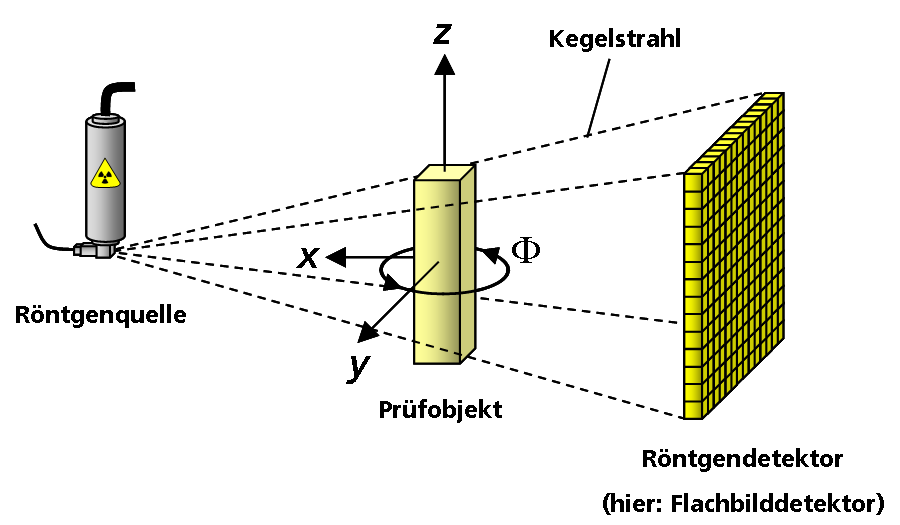
\includegraphics[height=\imheight]{./images/3D_Computed_Tomography}
%	\source{w.wiki/7g3}{\ccbysa}
%\end{frame}

\section{Examples}
\begin{frame}
	\frametitle{Examples}
	\centering
	\only<1>{%
		\pgfmathsetlength{\imagewidth}{0.9\linewidth}%
		\pgfmathsetlength{\imagescale}{\imagewidth/3295}%
		\def\x{2036}% scalebar-x starting at golden ratio of image width of 3295px = 2036
		\def\y{1343}% scalebar-y at 90% of image height of 1492px = 1343
		\begin{tikzpicture}[x=\imagescale,y=-\imagescale]
			\node[anchor=north west, inner sep=0pt, outer sep=0pt] at (0,0) {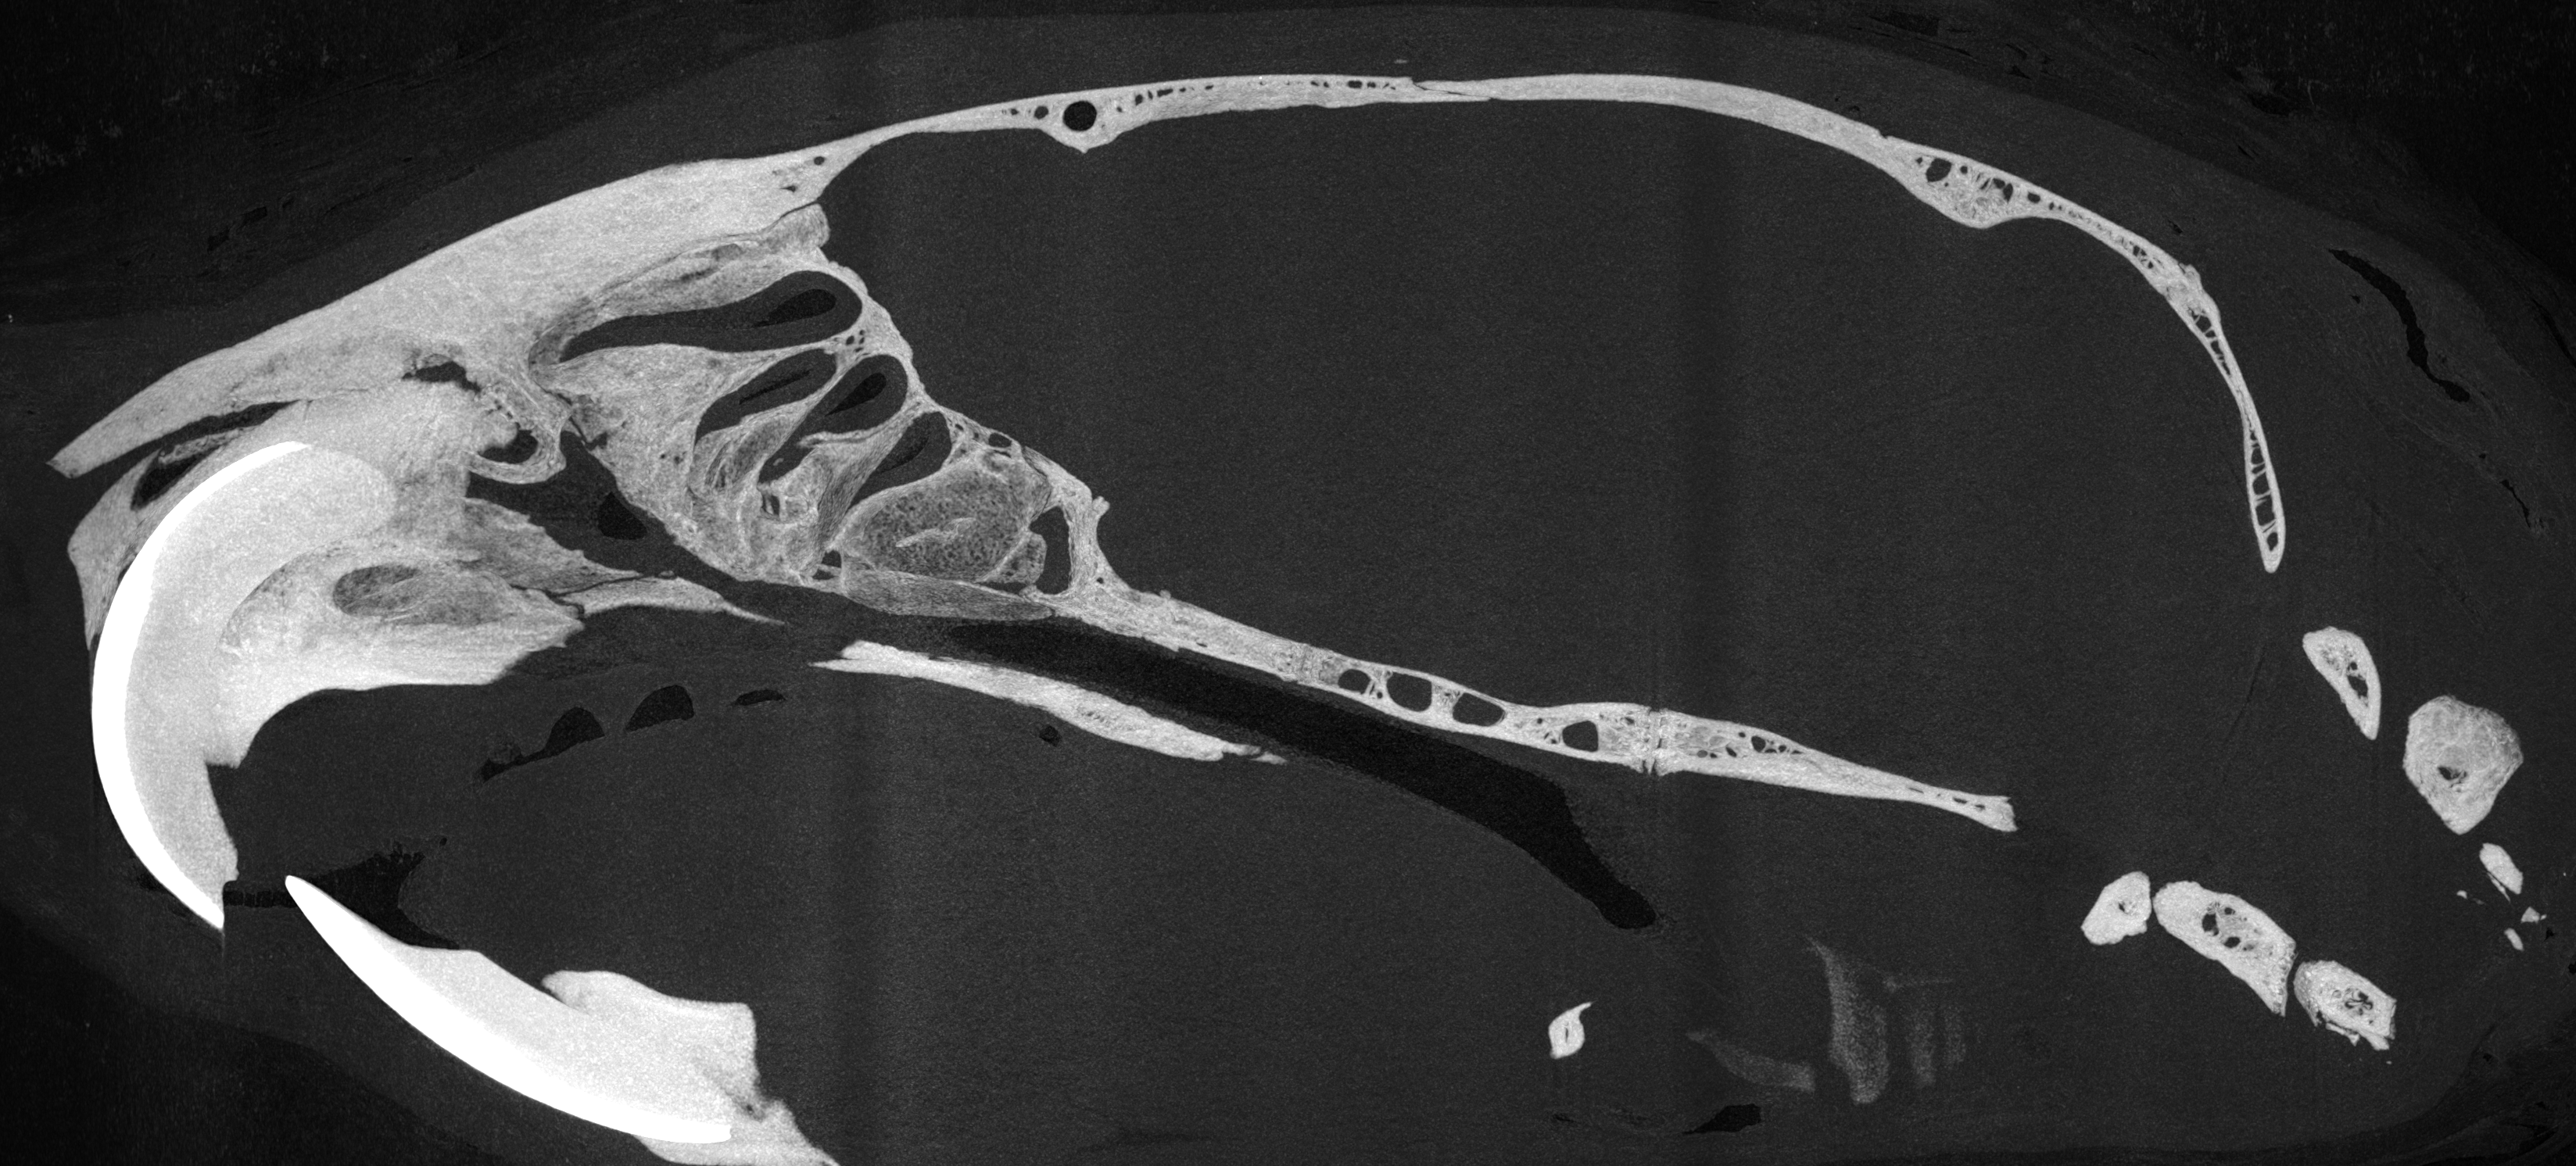
\includegraphics[width=\imagewidth]{./images/Mouse1265_resliced_MIP500um}};
			% 3295.000px = 26.2282mm -> 100px = 796.000um -> 62.814px = 500um, 12.563px = 100um
			%\draw[|-|,blue,thick] (0,746) -- (3295,746) node [sloped,midway,above,fill=white,semitransparent,text opacity=1] {\SI{26.2282}{\milli\meter} (3295px) TEMPORARY!};
			\draw[|-|,white,shadowed] (\x,\y) -- (\x+628.14,\y) node [midway,above] {\shadowtext{\SI{5}{\milli\meter}}};
		\end{tikzpicture}%
	}%
	\only<2>{%
		\pgfmathsetlength{\imagewidth}{0.618\linewidth}%
		\pgfmathsetlength{\imagescale}{\imagewidth/690}%
		\def\x{426}% scalebar-x starting at golden ratio of image width of 690px = 426
		\def\y{421}% scalebar-y at 90% of image height of 468px = 421
		\begin{tikzpicture}[x=\imagescale,y=-\imagescale]
			\node[anchor=north west, inner sep=0pt, outer sep=0pt] at (0,0) {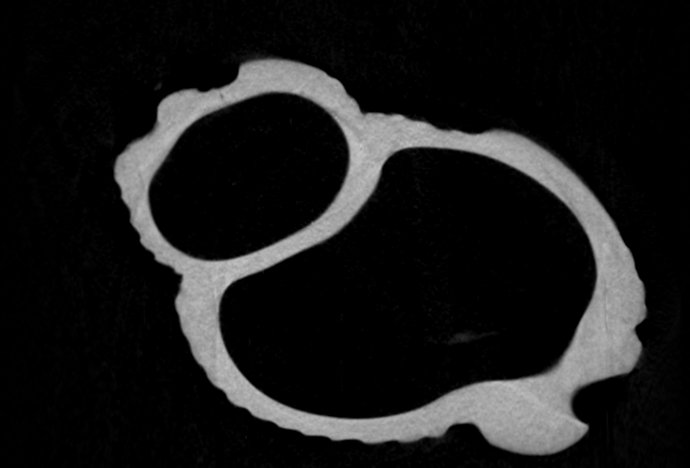
\includegraphics[width=\imagewidth]{./movies/shell/Muschel_klein0150}};
			% 690.000px = 7.452000000000001mm -> 100px = 1080.000um -> 46.296px = 500um, 9.259px = 100um
			%\draw[|-|,blue,thick] (0,234) -- (690,234) node [sloped,midway,above,fill=white,semitransparent,text opacity=1] {\SI{7.452000000000001}{\milli\meter} (690px) TEMPORARY!};
			\draw[|-|,white,shadowed] (\x,\y) -- (\x+92.59,\y) node [midway,above] {\shadowtext{\SI{1}{\milli\meter}}};
		\end{tikzpicture}%
	}
	\only<3>{%
		\animategraphics[autoplay,loop,width=0.618\linewidth,every=\everyframe]{24}{./movies/shell/Muschel_klein}{0150}{431}
	}
	\only<4>{%
		\pgfmathsetlength{\imagewidth}{0.42\linewidth}%
		\pgfmathsetlength{\imagescale}{\imagewidth/1224}%
		\def\x{756}% scalebar-x starting at golden ratio of image width of 1224px = 756
		\def\y{1102}% scalebar-y at 90% of image height of 1224px = 1102
		\begin{tikzpicture}[x=\imagescale,y=-\imagescale]
			\node[anchor=north west, inner sep=0pt, outer sep=0pt] at (0,0) {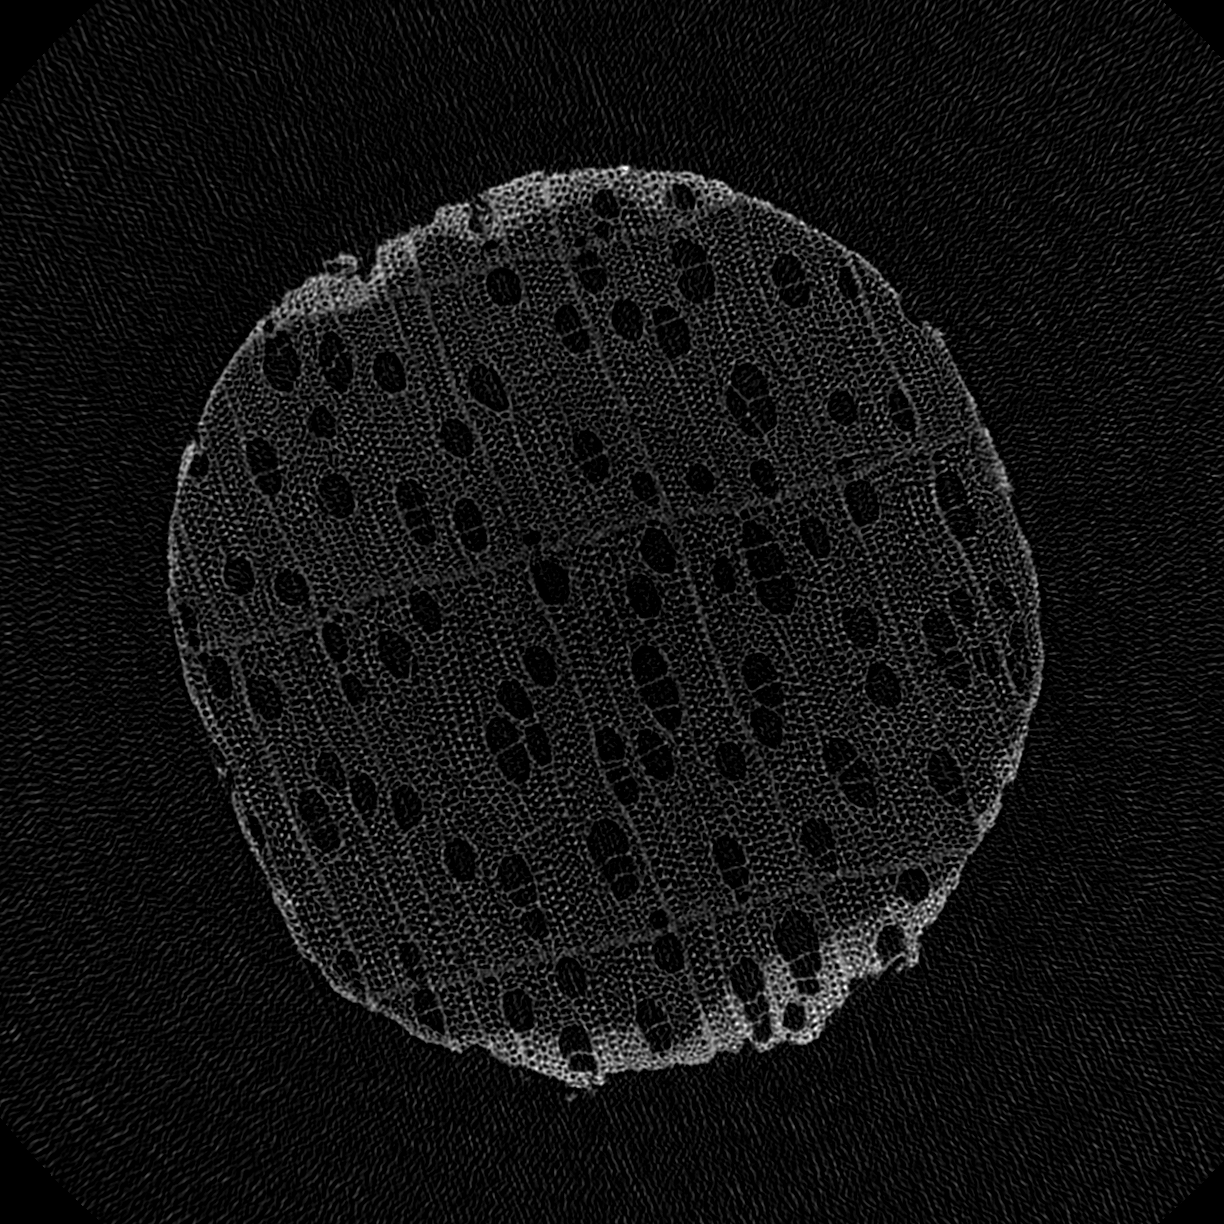
\includegraphics[width=\imagewidth]{./images/Toothpick_rec00000555}};
			% 1224.000px = 2.754mm -> 100px = 225.000um -> 222.222px = 500um, 44.444px = 100um
			%\draw[|-|,blue,thick] (0,612) -- (1224,612) node [sloped,midway,above,fill=white,semitransparent,text opacity=1] {\SI{2.754}{\milli\meter} (1224px) TEMPORARY!};
			\draw[|-|,white,shadowed] (\x,\y) -- (\x+222.222,\y) node [midway,above] {\shadowtext{\SI{500}{\micro\meter}}};
		\end{tikzpicture}%
	}
	\only<5>{%
		\pgfmathsetlength{\imagewidth}{0.55\linewidth}%
		\pgfmathsetlength{\imagescale}{\imagewidth/708}%
		\def\x{438+150}% scalebar-x starting at golden ratio of image width of 708px = 438
		\def\y{463}% scalebar-y at 90% of image height of 514px = 463
		\begin{tikzpicture}[x=\imagescale,y=-\imagescale]
			\node[anchor=north west, inner sep=0pt, outer sep=0pt] at (0,0) {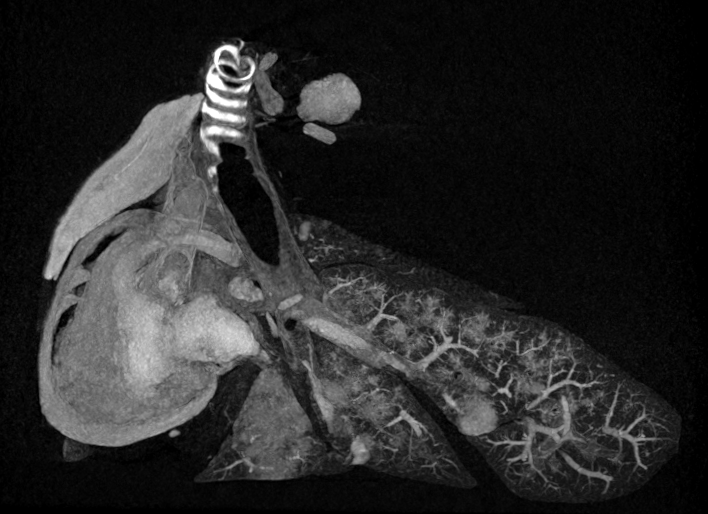
\includegraphics[width=\imagewidth]{./images/KP-TNIKWT2_rec_reslice_MIP500um}};
			% 708.000px = 15.292800000000002mm -> 100px = 2160.000um -> 23.148px = 500um, 4.630px = 100um
			%\draw[|-|,blue,thick] (0,257) -- (708,257) node [sloped,midway,above,fill=white,semitransparent,text opacity=1] {\SI{15.292800000000002}{\milli\meter} (708px) TEMPORARY!};
			\draw[|-|,white,shadowed] (\x,\y) -- (\x+46.3,\y) node [midway,above] {\shadowtext{\SI{1}{\milli\meter}}};
		\end{tikzpicture}%
	}
\end{frame}

\section{A scan, from start to finish}
\begin{frame}
	\frametitle{Projections}
	\centering
	% Movie frames generated with https://github.com/habi/Lecture.Microtomography/blob/master/Notebooks/FromProjectionsToReconstructions.ipynb
	\animategraphics[autoplay,loop,height=\imheight,every=\everyframe]{24}{./movies/scan/projections/KP-TNIKWT02_240_projections_of_940_800_px_}{000}{313}
\end{frame}

%\begin{frame}
%	\frametitle{Projections}
%	\begin{itemize}
%		\item A (micro-focus) x-ray source illuminates the object
%		\item The x-rays penetrate the sample and are attenuated
%		\item A scintillator converts the x-rays to visible light
%		\item A (planar) x-ray detector collects (magnified) projection images.
%		\item The projections are recorded on disk
%	\end{itemize}
%\end{frame}

\begin{frame}
	\frametitle{Reconstructions}
	\centering
	% Movie frames generated with https://github.com/habi/Lecture.Microtomography/blob/master/Notebooks/FromProjectionsToReconstructions.ipynb
	\animategraphics[autoplay,palindrome,height=\imheight,every=\everyframe]{24}{./movies/scan/reconstructions/KP-TNIKWT02_240_reconstructions_of_556_800_px_}{000}{277}
\end{frame}

%\begin{frame}
%	\frametitle{Reconstructions}
%	\begin{itemize}
%		\item Based on hundreds of angular views acquired while the object rotates, a computer synthesizes a stack of virtual cross section slices through the object.
%		\item Radon Transformation
%		\item Filtered back projection
%		\item Fan beam reconstruction
%		\item Corrections (beam hardening, etc.)
%		\item Writing to stack
%	\end{itemize}
%\end{frame}

\begin{frame}
	\frametitle{Visualization}
	\begin{tikzpicture}[remember picture,overlay]%
	\node at (current page.center){%
		\animategraphics[autoplay,loop,height=\paperheight,every=\everyframe]{24}{./movies/scan/visualization/lung}{000}{240}%
		};%
	\end{tikzpicture}%
\end{frame}

%\begin{frame}
%	\frametitle{Visualization}
%	\begin{itemize}
%		\item Based on the reconstructions the computer synthesizes a three-dimensional view of the scanned sample
%	\end{itemize}
%\end{frame}

\section{What about those teeth?}
\begin{frame}
	\frametitle{Tooth morphology}
	\begin{tikzpicture}[remember picture,overlay]%
		\node at (current page.center){%
			\animategraphics[autoplay,width=\paperwidth,every=\everyframe]{24}{./movies/tooth045/full/image0}{000}{474}%
			};%
	\end{tikzpicture}%
\end{frame}

\begin{frame}
	\frametitle{Internal morphology of human teeth}
	Collaboration with ZMK
	\begin{itemize}
		\item Numbers instead of just pretty images
		\item Segmentation
		\item (Unbiased) Characterization
		\item Reproducible and automated image analysis (\href{https://www.python.org/}{\faPython} in \href{https://jupyter.org/}{Jupyter}~\cite{Kluyver2016})
	\end{itemize}
\end{frame}

\subsection{Protocol}
\renewcommand{\imwidth}{\columnwidth}
\begin{frame}
	\frametitle{How?}
	\begin{columns}
		\begin{column}{0.49\linewidth}
			\begin{itemize}
				\item<1-> 104 extracted human permanent mandibular canines
				\item<2-> \uct imaging
				\item<4-> Morphology
				\begin{itemize}
					\item<4-> Root canal  morphology, according to~\citeauthor{Briseno-Marroquin2015}~\cite{Briseno-Marroquin2015}
					\item<5-> Foramen geometry and size, according to~\citeauthor{Wolf2017}~\cite{Wolf2017}
				\end{itemize}		
				\item<6-> \emph{Reproducible} analysis~\cite{Haberthur2020a}\onslide<7>{, \eg you can \href{https://mybinder.org/v2/gh/habi/zmk-tooth-cohort/master?filepath=ToothAnalysis.ipynb}{click a button to double-check} or \href{https://nbviewer.jupyter.org/github/habi/zmk-tooth-cohort/blob/master/ToothAnalysis.ipynb}{view it yourself}}
			\end{itemize}
		\end{column}
		\begin{column}{0.49\linewidth}
			\only<1>{%
				\centering
				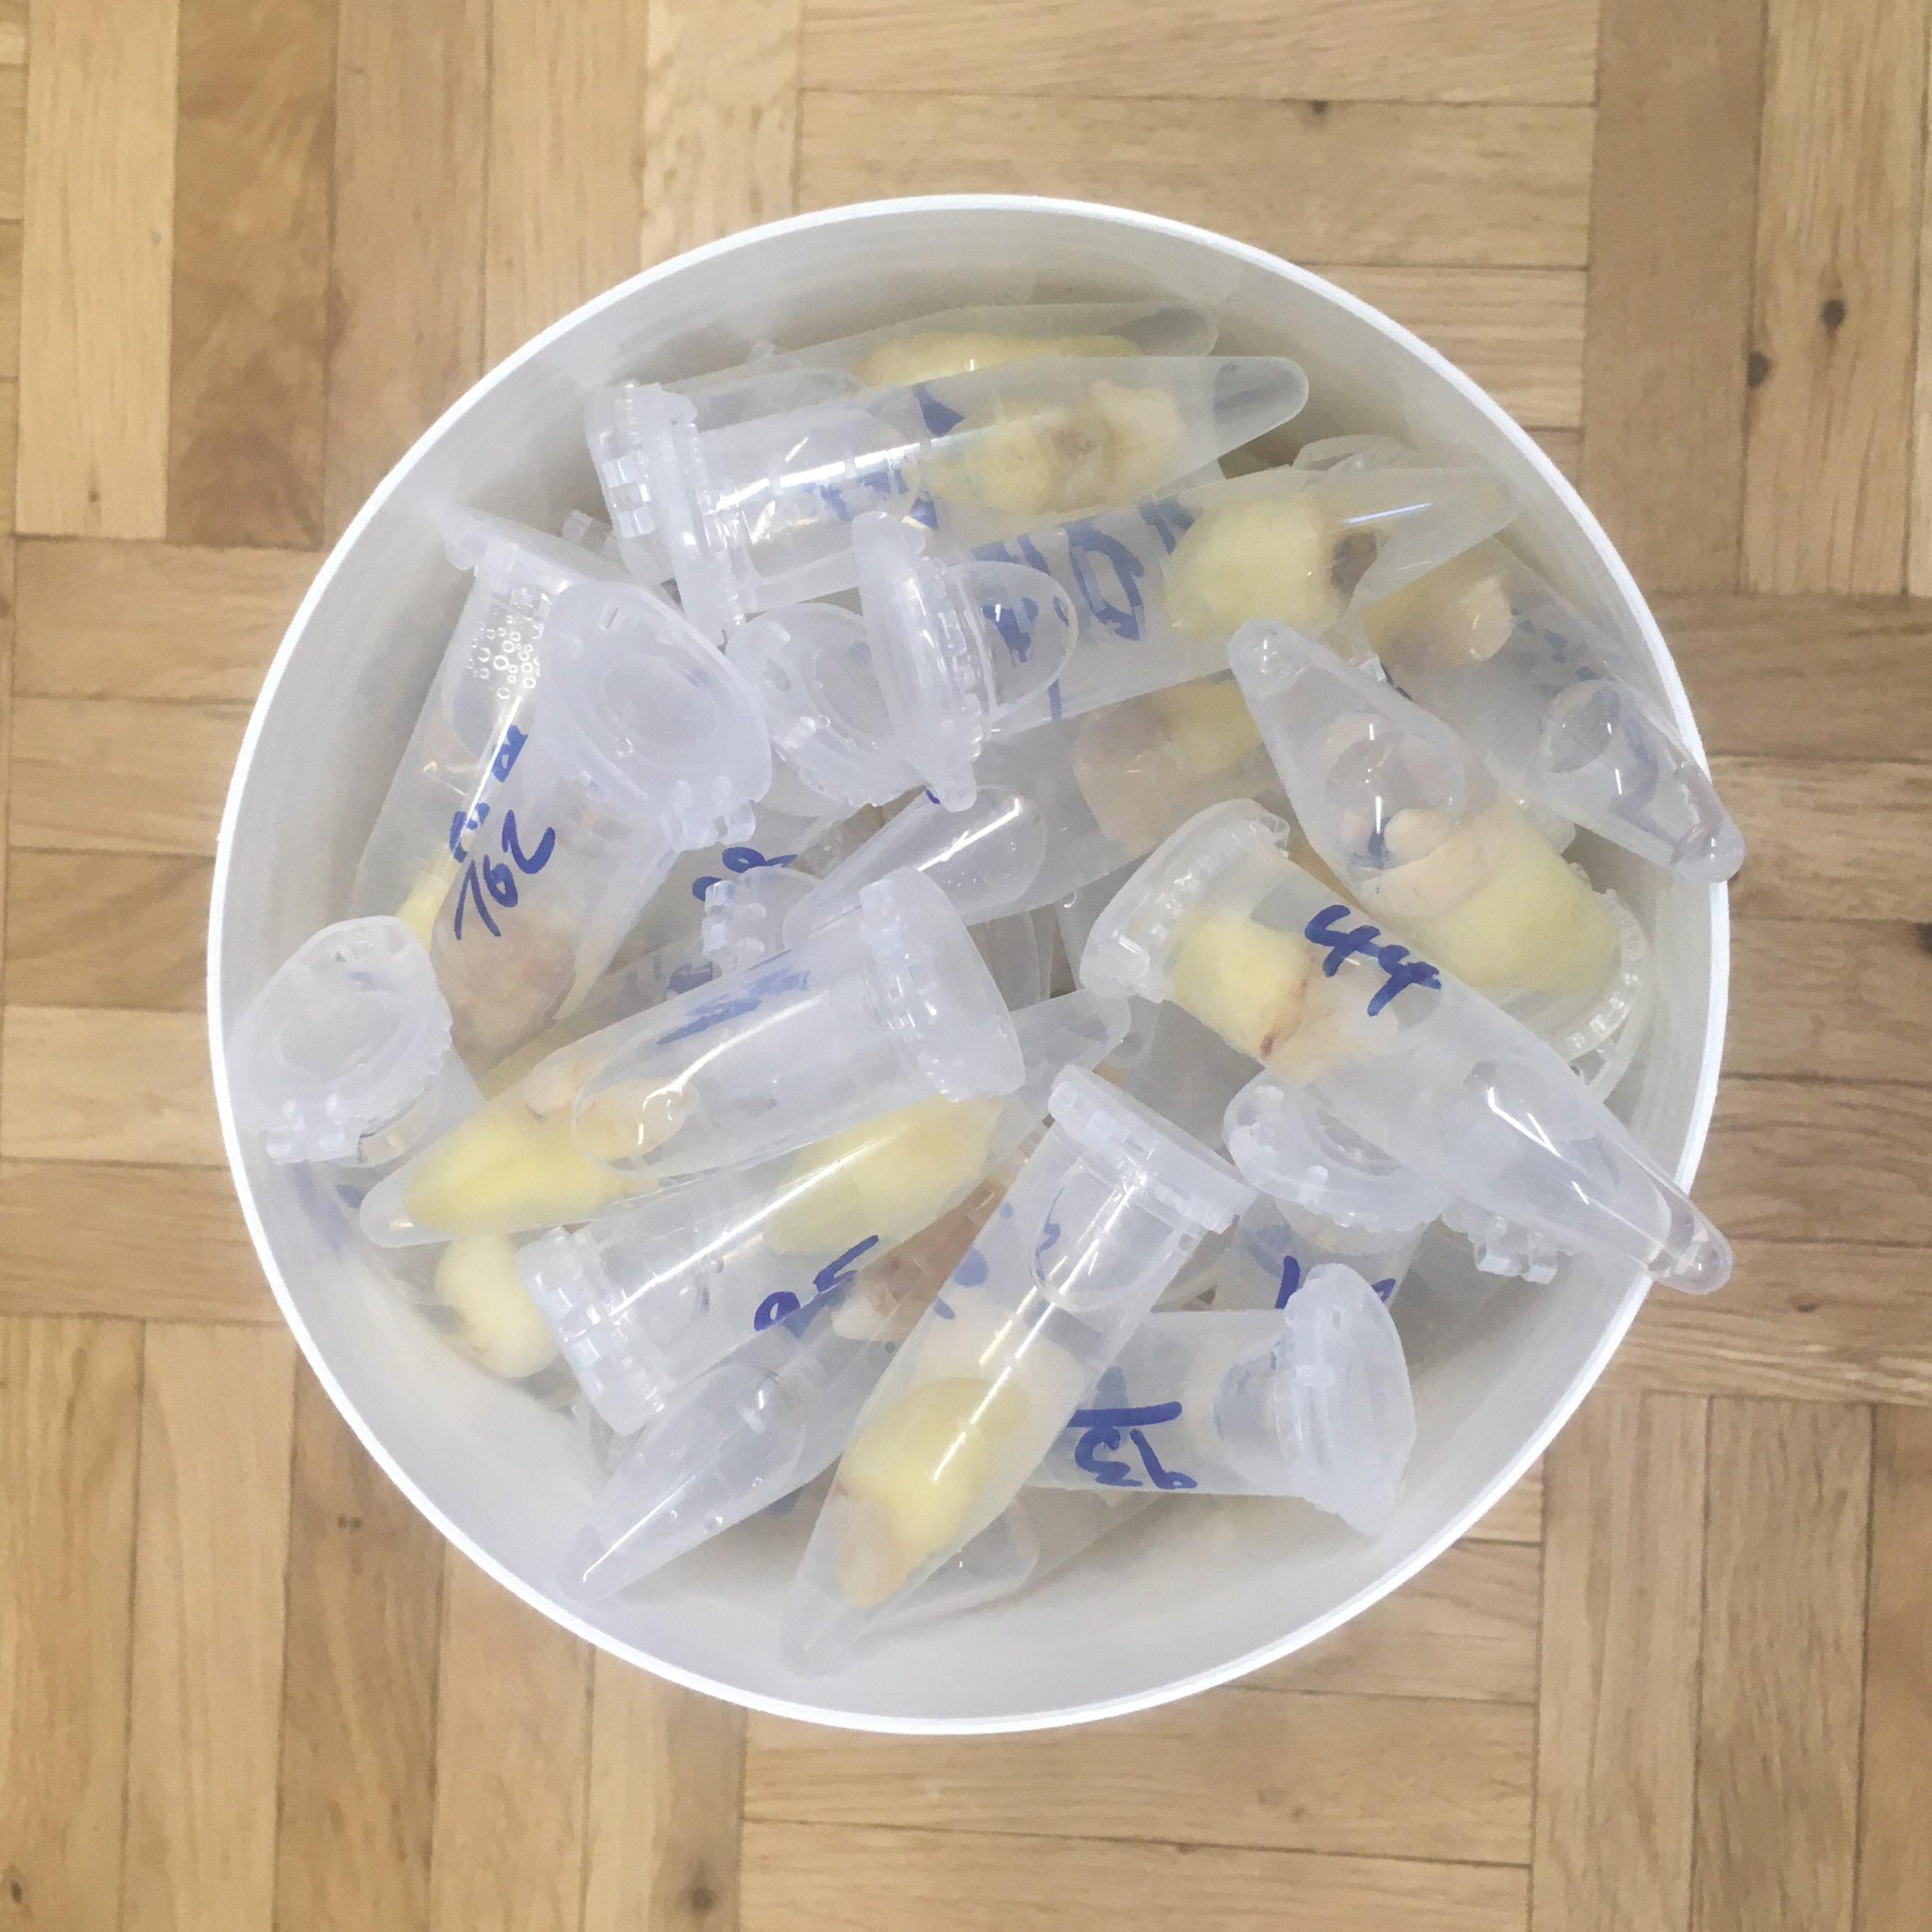
\includegraphics[height=\imheight]{./images/bucketofteeth}%
				}%
			\only<2>{%
				\lstinputlisting[linerange={2-4,15-15,17-19,28-30,36-37,40-40,44-44,53-54}]{./logfiles/Tooth045.log}%
				}%
			\only<3>{%
				\emph{Sample changer} on the SkyScan 1272\newline
				In total:
				\begin{itemize}
					\item 13 days of \emph{continuous} \uct scanning
					\item \SI{819}{\giga\byte} of raw data\newline\num{230648} TIFF projections
					\item \SI{326}{\giga\byte} data as input for analysis\newline\num{282062} PNG reconstructions
				\end{itemize}					
					}%		
			\only<4>{%
				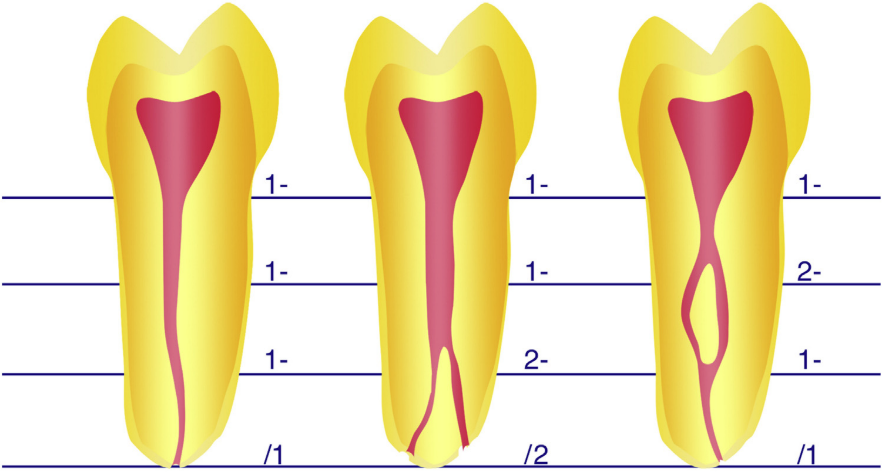
\includegraphics[width=\textwidth]{./images/briseno}%
				\sourcecite{Briseno-Marroquin2015}{Fig.~2}%
				}%
			\only<5>{%
				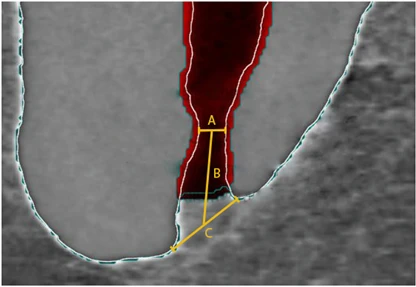
\includegraphics[width=\textwidth]{./images/foramen}%
				\sourcecite{Wolf2017}{Fig.~1}%
				}%		
			\only<6>{%
				\animategraphics[loop,autoplay,width=\linewidth,every=\everyframe]{24}{./movies/coder/coder-}{0}{133}%
				\source{gph.is/2nqkple}{}%
				}%
			\only<7>{%
				\centering
				\href{https://mybinder.org/v2/gh/habi/zmk-tooth-cohort/master?filepath=ToothAnalysis.ipynb}{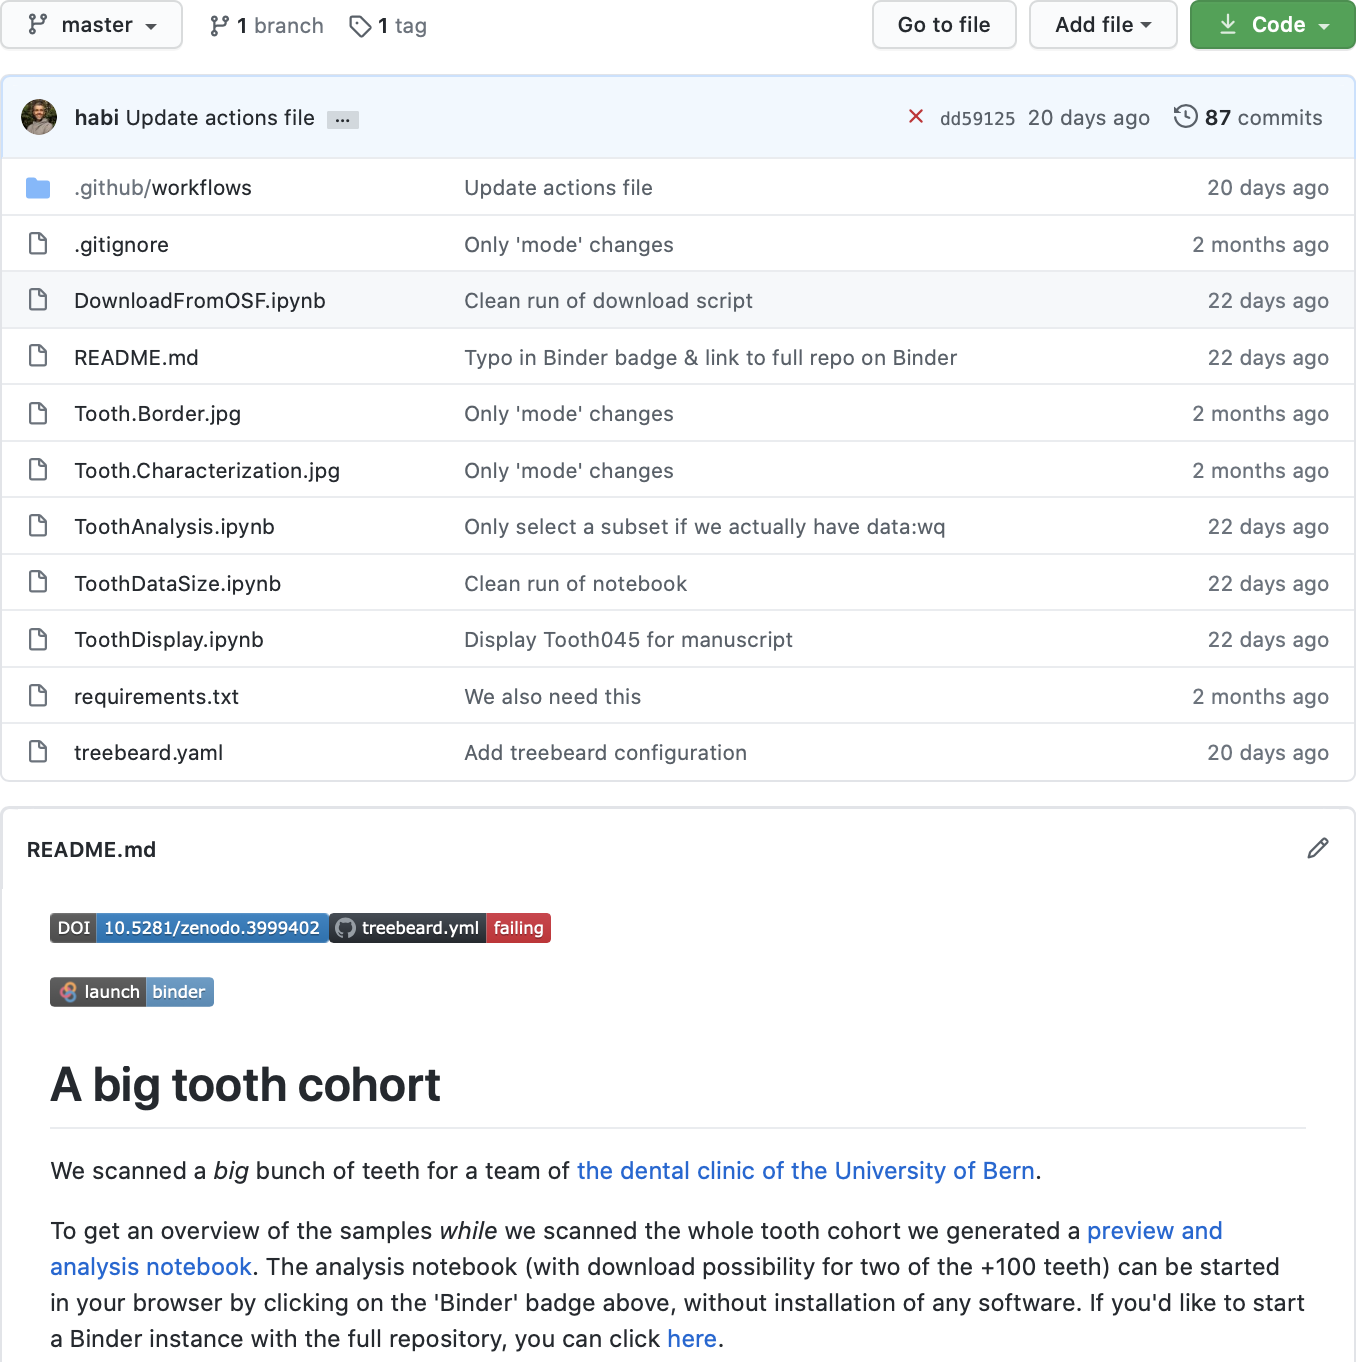
\includegraphics[height=\imheight]{./images/binder}}%
				}%
		\end{column}
	\end{columns}
\end{frame}

\subsection{\uct imaging}
\begin{frame}
	\frametitle{\uct imaging}
	\centering
	\includegraphics<1>[height=\imheight]{./images/{{ScanOverviews.104}}}%
	\includegraphics<2>[height=\imheight]{./images/{{ScanOverviews.24}}}%
\end{frame}	
	
\subsection{(hands-off) Image processing}
\begin{frame}
	\frametitle{Dataset cropping}
	\begin{columns}
		\begin{column}{0.309\linewidth}	
			\begin{itemize}
				\item Full datasets: \SI{326}{\giga\byte}
				\item \uncover<2->{Cropped: \SI{115}{\giga\byte}}
			\end{itemize}
		\end{column}	
		\begin{column}{0.618\linewidth}
			\centering
			\renewcommand{\imwidth}{\columnwidth}%				
			\only<1>{%
				\pgfmathsetlength{\imagewidth}{\imwidth}%
				\pgfmathsetlength{\imagescale}{\imagewidth/2585}%
				\def\x{1598}% scalebar-x starting at golden ratio of image width of 2585px = 1598
				\def\y{1469}% scalebar-y at 90% of image height of 1632px = 1469
				\begin{tikzpicture}[x=\imagescale,y=-\imagescale]
					\node[anchor=north west, inner sep=0pt, outer sep=0pt] at (0,0) {\includegraphics[width=\imagewidth]{./images/tooth045/{{Tooth045.mip.rec}}}};
					% 2585.000px = 25.849963810000002mm -> 100px = 999.999um -> 50.000px = 500um, 10.000px = 100um
					\draw[|-|,white,shadowed] (\x,\y) -- (\x+500,\y) node [midway,above] {\shadowtext{\SI{5}{\milli\meter}}};
				\end{tikzpicture}%
				}%
			\only<2>{%
				\pgfmathsetlength{\imagewidth}{\imwidth}%
				\pgfmathsetlength{\imagescale}{\imagewidth/2391}%
				\def\x{1478}% scalebar-x starting at golden ratio of image width of 2391px = 1478
				\def\y{547}% scalebar-y at 90% of image height of 608px = 547
				\begin{tikzpicture}[x=\imagescale,y=-\imagescale]
					\node[anchor=north west, inner sep=0pt, outer sep=0pt] at (0,0) {\includegraphics[width=\imagewidth]{./images/tooth045/{{Tooth045.mip.rec.crop}}}};
					% 2391.000px = 23.909966526mm -> 100px = 999.999um -> 50.000px = 500um, 10.000px = 100um
					\draw[|-|,white,shadowed] (\x,\y) -- (\x+500,\y) node [midway,above] {\shadowtext{\SI{5}{\milli\meter}}};
				\end{tikzpicture}%
				}%
		\end{column}	
	\end{columns}		
\end{frame}

\begin{frame}
	\frametitle{Tooth morphology}
	\begin{tikzpicture}[remember picture,overlay]%
		\node at (current page.center){%
			\only<1>{\animategraphics[autoplay,width=\paperwidth,every=\everyframe]{24}{./movies/tooth045/full/image0}{000}{474}}%
			\only<2>{\animategraphics[autoplay,width=\paperwidth,every=\everyframe]{24}{./movies/tooth045/full-slices/image0}{000}{466}}%
			};%
	\end{tikzpicture}%
\end{frame}

\begin{frame}
	\frametitle{Detection of enamel-dentin border}
	\centering
	\only<1>{%
		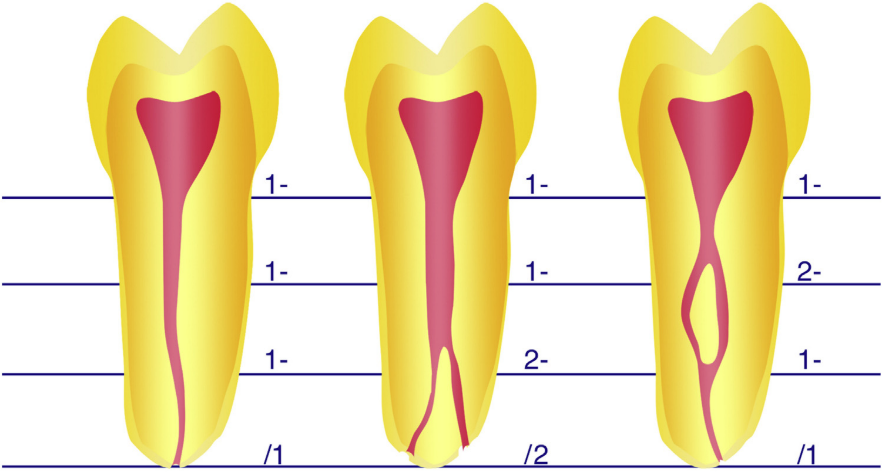
\includegraphics[height=\imheight]{./images/briseno}%
		\sourcecite{Briseno-Marroquin2015}{Fig.~2}%
		}
	\only<2>{%
		\includegraphics[height=\imheight]{./images/tooth045/{{Tooth045.ExtractedSlices}}}%
		}
	\only<3>{%
		\includegraphics[width=\linewidth]{./images/tooth045/{{Tooth045.Briseno}}}%
		}
\end{frame}

\begin{frame}
	\frametitle{Extraction of pulpa}
	\begin{tikzpicture}[remember picture,overlay]%
		\node at (current page.center){%
			\only<1>{\animategraphics[loop,autoplay,width=\paperwidth,every=\everyframe]{24}{./movies/tooth045/transparent-slices/image0}{000}{473}}%
			\only<2>{\animategraphics[loop,autoplay,width=\paperwidth,every=\everyframe]{24}{./movies/tooth045/pulpa/image0}{000}{413}}%
			};%
	\end{tikzpicture}%
\end{frame}

\begin{frame}
	\frametitle{Analysis of the physiological foramen geometry}
	\centering
	\only<1>{%
		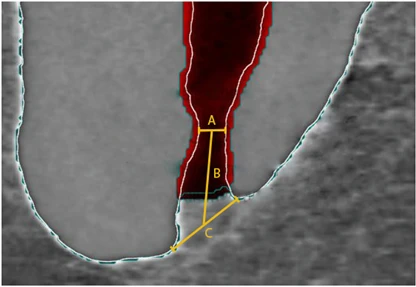
\includegraphics[height=\imheight]{./images/foramen}%
		\sourcecite{Wolf2017}{Fig.~1}%
		}%
	\only<2>{%
		\animategraphics[palindrome,autoplay,height=\imheight,every=\everyframe]{24}{./movies/tooth045/edt-axial/Tooth045_EDT_Axial_}{100}{199}%
		}%
	\only<3>{%
		\animategraphics[palindrome,autoplay,height=\imheight,every=\everyframe]{24}{./movies/tooth045/edt-coronal/Tooth045_EDT_Coronal_}{123}{213}%
		}		
\end{frame}

\section{\emph{Take to lunch}-message}
\begin{frame}
	\frametitle{Conclusion}
	\begin{itemize}
		\item Efficient use of time
		\item Reproducible analysis with \emph{free and open-source software}
		\item Objective analysis, \eg no operator bias
		\item More teeth does not mean more (analysis) work
	\end{itemize}
\end{frame}

\begin{frame}
	\frametitle{Thanks!}
	\begin{columns}
		\begin{column}{0.5\linewidth}
		\begin{itemize}
			\item Topographic and clinical Anatomy
				\begin{itemize}
					\item Valentin Djonov, Ruslan Hlushchuk, Oleksiy-Zakhar Khoma and Jennifer Fazzari
				\end{itemize}
			\item zmk bern – Zahnmedizinische Kliniken
				\begin{itemize}
					\item Thomas G.\ Wolf, Andrea Anderegg and Michael Stiebritz
				\end{itemize}				
			\item SNF
			\item<2-> You, for listening to me
			\item<3-> \href{https://twitter.com/jackiantonovich/status/1195699076056178691}{What questions do you have for me} and \href{https://twitter.com/ElaineLuther/status/1195708328854331392}{what can I clarify for you}?
		\end{itemize}
		\end{column}
		\begin{column}{0.5\linewidth}
			\centering
			\includegraphics<1->[height=\imheight]{./images/team}
		\end{column}
	\end{columns}
	\only<4>{%
		\begin{tikzpicture}[remember picture,overlay]%
			\node at (current page.center){%
				\animategraphics[loop,autoplay,width=\paperwidth,every=\everyframe]{24}{./movies/tooth045/full-slices/image0}{000}{466}%
				};%
		\end{tikzpicture}%
	}%
\end{frame}

\begin{frame}
	\frametitle{References \& \href{https://en.wikipedia.org/wiki/Colophon_(publishing)}{Colophon}}
	\begin{columns}
		\begin{column}{0.6\linewidth}
			% Make the references continuously smaller :)
			%\renewcommand*{\bibfont}{\small}
			%\renewcommand*{\bibfont}{\footnotesize}
			%\renewcommand*{\bibfont}{\scriptsize}
			\renewcommand*{\bibfont}{\tiny}
			\setbeamertemplate{bibliography item}{\insertbiblabel}
			\printbibliography
		\end{column}	
		\begin{column}{0.4\linewidth}
			\begin{itemize}
				\item This \textsc{beamer} presentation was crafted in \LaTeX\xspace with the (slightly adapted) \href{http://intern.unibe.ch/dienstleistungen/corporate_design_und_vorlagen/praesentationen/index_ger.html}{template from \emph{Corporate Design und Vorlagen} of the University of Bern}.
				\begin{itemize}
					\item \href{https://github.com/habi/20201112_Anatomie_Seminar}{Fully reproducible source: git.io/JkJ5w}
				\end{itemize}
				\item Did you spot an error?
				\begin{itemize}
					\item \href{https://github.com/habi/20201112_Anatomie_Seminar/issues}{File an issue: git.io/JkJ5K}
					\item \href{mailto:haberthuer@ana.unibe.ch?subject=Error\%20in\%20the\%20seminar\%20presentation\&body=https://xkcd.com/386/}{Send me an email: haberthuer@ana.unibe.ch}
				\end{itemize}
			\end{itemize}
		\end{column}
	\end{columns}
\end{frame}

\end{document}